% arara: lualatex: { synctex: on, shell: off }
% arara: biber
% arara: lualatex: { synctex: on, shell: off }
% arara: sumatrapdf
\documentclass[12pt,letterpaper,oneside,draft]{book}

\usepackage{luacode}
\edef \user{\directlua{tex.sprint(os.getenv('USERNAME'))}}

\usepackage{fancyvrb}
\usepackage{color}

\makeatletter
\def\PY@reset{\let\PY@it=\relax \let\PY@bf=\relax%
    \let\PY@ul=\relax \let\PY@tc=\relax%
    \let\PY@bc=\relax \let\PY@ff=\relax}
\def\PY@tok#1{\csname PY@tok@#1\endcsname}
\def\PY@toks#1+{\ifx\relax#1\empty\else%
    \PY@tok{#1}\expandafter\PY@toks\fi}
\def\PY@do#1{\PY@bc{\PY@tc{\PY@ul{%
    \PY@it{\PY@bf{\PY@ff{#1}}}}}}}
\def\PY#1#2{\PY@reset\PY@toks#1+\relax+\PY@do{#2}}

\expandafter\def\csname PY@tok@gu\endcsname{\let\PY@bf=\textbf\def\PY@tc##1{\textcolor[rgb]{0.50,0.00,0.50}{##1}}}
\expandafter\def\csname PY@tok@gt\endcsname{\def\PY@tc##1{\textcolor[rgb]{0.00,0.27,0.87}{##1}}}
\expandafter\def\csname PY@tok@gs\endcsname{\let\PY@bf=\textbf}
\expandafter\def\csname PY@tok@gr\endcsname{\def\PY@tc##1{\textcolor[rgb]{1.00,0.00,0.00}{##1}}}
\expandafter\def\csname PY@tok@cm\endcsname{\def\PY@tc##1{\textcolor[rgb]{0.00,0.53,0.00}{##1}}}
\expandafter\def\csname PY@tok@gp\endcsname{\let\PY@bf=\textbf\def\PY@tc##1{\textcolor[rgb]{0.78,0.36,0.04}{##1}}}
\expandafter\def\csname PY@tok@m\endcsname{\let\PY@bf=\textbf\def\PY@tc##1{\textcolor[rgb]{1.00,0.00,0.00}{##1}}}
\expandafter\def\csname PY@tok@mh\endcsname{\let\PY@bf=\textbf\def\PY@tc##1{\textcolor[rgb]{1.00,0.00,0.00}{##1}}}
\expandafter\def\csname PY@tok@cs\endcsname{\def\PY@tc##1{\textcolor[rgb]{0.00,0.53,0.00}{##1}}}
\expandafter\def\csname PY@tok@ge\endcsname{\let\PY@it=\textit}
\expandafter\def\csname PY@tok@gd\endcsname{\def\PY@tc##1{\textcolor[rgb]{0.63,0.00,0.00}{##1}}}
\expandafter\def\csname PY@tok@il\endcsname{\let\PY@bf=\textbf\def\PY@tc##1{\textcolor[rgb]{1.00,0.00,0.00}{##1}}}
\expandafter\def\csname PY@tok@go\endcsname{\def\PY@tc##1{\textcolor[rgb]{0.53,0.53,0.53}{##1}}}
\expandafter\def\csname PY@tok@cp\endcsname{\def\PY@tc##1{\textcolor[rgb]{0.00,0.53,0.00}{##1}}}
\expandafter\def\csname PY@tok@gi\endcsname{\def\PY@tc##1{\textcolor[rgb]{0.00,0.63,0.00}{##1}}}
\expandafter\def\csname PY@tok@gh\endcsname{\let\PY@bf=\textbf\def\PY@tc##1{\textcolor[rgb]{0.00,0.00,0.50}{##1}}}
\expandafter\def\csname PY@tok@s2\endcsname{\def\PY@tc##1{\textcolor[rgb]{0.44,0.44,0.44}{##1}}}
\expandafter\def\csname PY@tok@nb\endcsname{\let\PY@bf=\textbf\def\PY@tc##1{\textcolor[rgb]{0.00,0.00,1.00}{##1}}}
\expandafter\def\csname PY@tok@nc\endcsname{\let\PY@bf=\textbf\def\PY@tc##1{\textcolor[rgb]{0.73,0.00,0.40}{##1}}}
\expandafter\def\csname PY@tok@si\endcsname{\def\PY@tc##1{\textcolor[rgb]{0.44,0.44,0.44}{##1}}\def\PY@bc##1{\setlength{\fboxsep}{0pt}\colorbox[rgb]{0.93,0.93,0.93}{\strut ##1}}}
\expandafter\def\csname PY@tok@nf\endcsname{\def\PY@tc##1{\textcolor[rgb]{1.00,0.08,0.58}{##1}}}
\expandafter\def\csname PY@tok@sh\endcsname{\def\PY@tc##1{\textcolor[rgb]{0.44,0.44,0.44}{##1}}}
\expandafter\def\csname PY@tok@s1\endcsname{\def\PY@tc##1{\textcolor[rgb]{0.44,0.44,0.44}{##1}}}
\expandafter\def\csname PY@tok@ow\endcsname{\let\PY@bf=\textbf\def\PY@tc##1{\textcolor[rgb]{0.00,0.00,1.00}{##1}}}
\expandafter\def\csname PY@tok@mf\endcsname{\let\PY@bf=\textbf\def\PY@tc##1{\textcolor[rgb]{1.00,0.00,0.00}{##1}}}
\expandafter\def\csname PY@tok@bp\endcsname{\let\PY@bf=\textbf\def\PY@tc##1{\textcolor[rgb]{0.00,0.00,1.00}{##1}}}
\expandafter\def\csname PY@tok@c1\endcsname{\def\PY@tc##1{\textcolor[rgb]{0.00,0.53,0.00}{##1}}}
\expandafter\def\csname PY@tok@kc\endcsname{\let\PY@bf=\textbf\def\PY@tc##1{\textcolor[rgb]{0.00,0.00,1.00}{##1}}}
\expandafter\def\csname PY@tok@c\endcsname{\def\PY@tc##1{\textcolor[rgb]{0.00,0.53,0.00}{##1}}}
\expandafter\def\csname PY@tok@sx\endcsname{\def\PY@tc##1{\textcolor[rgb]{0.87,0.13,0.00}{##1}}}
\expandafter\def\csname PY@tok@err\endcsname{\def\PY@tc##1{\textcolor[rgb]{1.00,0.00,0.00}{##1}}\def\PY@bc##1{\setlength{\fboxsep}{0pt}\colorbox[rgb]{1.00,0.67,0.67}{\strut ##1}}}
\expandafter\def\csname PY@tok@kd\endcsname{\let\PY@bf=\textbf\def\PY@tc##1{\textcolor[rgb]{0.00,0.00,1.00}{##1}}}
\expandafter\def\csname PY@tok@ss\endcsname{\def\PY@tc##1{\textcolor[rgb]{0.67,0.40,0.00}{##1}}}
\expandafter\def\csname PY@tok@sr\endcsname{\def\PY@tc##1{\textcolor[rgb]{0.00,0.00,0.00}{##1}}\def\PY@bc##1{\setlength{\fboxsep}{0pt}\colorbox[rgb]{1.00,0.94,1.00}{\strut ##1}}}
\expandafter\def\csname PY@tok@mo\endcsname{\let\PY@bf=\textbf\def\PY@tc##1{\textcolor[rgb]{1.00,0.00,0.00}{##1}}}
\expandafter\def\csname PY@tok@mi\endcsname{\let\PY@bf=\textbf\def\PY@tc##1{\textcolor[rgb]{1.00,0.00,0.00}{##1}}}
\expandafter\def\csname PY@tok@kn\endcsname{\let\PY@bf=\textbf\def\PY@tc##1{\textcolor[rgb]{0.00,0.00,1.00}{##1}}}
\expandafter\def\csname PY@tok@o\endcsname{\def\PY@tc##1{\textcolor[rgb]{0.20,0.20,0.20}{##1}}}
\expandafter\def\csname PY@tok@kr\endcsname{\let\PY@bf=\textbf\def\PY@tc##1{\textcolor[rgb]{0.00,0.00,1.00}{##1}}}
\expandafter\def\csname PY@tok@s\endcsname{\def\PY@tc##1{\textcolor[rgb]{0.44,0.44,0.44}{##1}}}
\expandafter\def\csname PY@tok@kp\endcsname{\let\PY@bf=\textbf\def\PY@tc##1{\textcolor[rgb]{0.00,0.00,1.00}{##1}}}
\expandafter\def\csname PY@tok@w\endcsname{\def\PY@tc##1{\textcolor[rgb]{0.73,0.73,0.73}{##1}}}
\expandafter\def\csname PY@tok@kt\endcsname{\let\PY@bf=\textbf\def\PY@tc##1{\textcolor[rgb]{0.00,0.00,1.00}{##1}}}
\expandafter\def\csname PY@tok@sc\endcsname{\def\PY@tc##1{\textcolor[rgb]{0.00,0.27,0.87}{##1}}}
\expandafter\def\csname PY@tok@sb\endcsname{\def\PY@tc##1{\textcolor[rgb]{0.44,0.44,0.44}{##1}}}
\expandafter\def\csname PY@tok@k\endcsname{\let\PY@bf=\textbf\def\PY@tc##1{\textcolor[rgb]{0.00,0.00,1.00}{##1}}}
\expandafter\def\csname PY@tok@se\endcsname{\let\PY@bf=\textbf\def\PY@tc##1{\textcolor[rgb]{0.40,0.40,0.40}{##1}}}
\expandafter\def\csname PY@tok@sd\endcsname{\def\PY@tc##1{\textcolor[rgb]{0.87,0.27,0.13}{##1}}}

\def\PYZbs{\char`\\}
\def\PYZus{\char`\_}
\def\PYZob{\char`\{}
\def\PYZcb{\char`\}}
\def\PYZca{\char`\^}
\def\PYZam{\char`\&}
\def\PYZlt{\char`\<}
\def\PYZgt{\char`\>}
\def\PYZsh{\char`\#}
\def\PYZpc{\char`\%}
\def\PYZdl{\char`\$}
\def\PYZhy{\char`\-}
\def\PYZsq{\char`\'}
\def\PYZdq{\char`\"}
\def\PYZti{\char`\~}
% for compatibility with earlier versions
\def\PYZat{@}
\def\PYZlb{[}
\def\PYZrb{]}
\makeatother

%Set the package to import preambles
\usepackage{subfiles}

%Load graphicx here to specify options
\usepackage[final]{graphicx}

%Set the document font
\usepackage[no-math]{fontspec}
\setmainfont[Ligatures=TeX]{Times New Roman}
\setmonofont{Inconsolata}

%Set the text to double spacing
%According to hyperref README,
%setspace should be loaded first
\usepackage[doublespacing]{setspace}

%Set a command to easily skip a line
\newcommand{\blankline}{\vspace*{\baselineskip}}

%Set up biblatex
\usepackage[
    backend=biber,
    % url=false,
    doi=true,
    sorting=none,
    sortcites=true,
    maxbibnames=6,
    minbibnames=6,
    maxcitenames=2,
    mincitenames=1,
    citestyle=numeric-comp,
    firstinits=true,
    isbn=false
]{biblatex}
\addbibresource{C:/Users/\user/Documents/Github/dissertation/library.bib}

%Remove the "In:" from before the journal title for articles
\renewbibmacro{in:}{%
  \ifentrytype{article}{}{\printtext{\bibstring{in}\intitlepunct}}}

%Change the name of the bibliography section to "References"
\DefineBibliographyStrings{english}{bibliography = {References}}

%Set the sort order of the names in each bibliography entry
\DeclareNameAlias{default}{last-first}

%Don't print the article title. To print the title, add #1 to the last {}
\DeclareFieldFormat[article,incollection,unpublished]{title}{}

%Add "vol." and "no." before volume and issue.
\DeclareFieldFormat[article]{volume}{\bibstring{volume}\addspace #1}
\DeclareFieldFormat[article]{number}{\bibstring{number}\addspace #1}

%Ensure that a comma follows abbreviated journal titles.
\DeclareFieldFormat{journaltitle}{\mkbibemph{#1}\isdot}

%Put a comma between the volume and issue instead of period.
\renewbibmacro*{volume+number+eid}{%
  \printfield{volume}%
  \setunit{\addcomma\space}%<---- was \setunit*{\adddot}%
  \printfield{number}%
  \setunit{\addcomma\space}%
  \printfield{eid}}

%Add a comma after the journal title.
\renewbibmacro*{journal+issuetitle}{%
  \usebibmacro{journal}%
  \setunit*{\addcomma\addspace}%<---- was \setunit*{\addspace}%
  \iffieldundef{series}
    {}
    {\newunit
     \printfield{series}%
     \setunit{\addspace}}%
  \usebibmacro{volume+number+eid}%
  \setunit{\addspace}%
  \usebibmacro{issue+date}%
  \setunit{\addcolon\space}%
  \usebibmacro{issue}%
  \newunit}

%Only print URL if doi is not present.
\DeclareFieldFormat{url}{%
  \iffieldundef{doi}{%
    \mkbibacro{URL}\addcolon\space\url{#1}%
  }{%
  }%
}
\DeclareFieldFormat{urldate}{%
  \iffieldundef{doi}{%
    \mkbibparens{\bibstring{urlseen}\space#1}%
  }{%
  }%
}

%Remove publisher from being printed.
\renewbibmacro*{publisher+location+date}{%
  \printlist{location}%
  \setunit*{\addcomma\space}%
  \usebibmacro{date}%
  \newunit}

%Fix in-text full citations
\DeclareCiteCommand{\fullcite}
  {\usebibmacro{prenote}}
  {\usedriver
     {\defcounter{minnames}{99}%
      \defcounter{maxnames}{99}}
     {\thefield{entrytype}}}
  {\multicitedelim}
  {\usebibmacro{postnote}}

%Use fancy tables.
\usepackage{booktabs}

%Set up todo notes in the PDF file
\usepackage{todonotes}

%Use and set up the caption package for nicer captions.
\usepackage{caption}
\DeclareCaptionLabelFormat{bf}{\textbf{#1 #2}}
\captionsetup{
    font=small ,
    labelsep=colon ,
    labelformat=bf ,
    figurewithin=chapter ,
    tablewithin=chapter ,
}

\usepackage{titlesec}
\usepackage{titletoc}

\titleformat{\chapter}[display]{\normalfont\Huge\bfseries}{Chapter \thechapter}{0.7em}{}
\titleformat{\section}{\normalfont\LARGE\bfseries}{\thesection}{0.5em}{}
\titleformat{\subsection}{\normalfont\Large\bfseries}{\thesubsection}{1em}{}
\titleformat{\subsubsection}{\normalfont\large\bfseries}{\thesubsubsection}{1em}{}

\titlecontents{chapter}[0pc]{}{\bfseries Chapter \thecontentslabel\quad}{}{\titlerule*[0.5pc]{.}\contentspage}
\titlecontents{section}[1em]{}{\thecontentslabel\quad}{}{\titlerule*[0.5pc]{.}\contentspage}
\titlecontents{subsection}[2em]{}{\thecontentslabel\quad}{}{\titlerule*[0.5pc]{.}\contentspage}
\titlecontents{subsubsection}[3em]{}{\thecontentslabel\quad}{}{\titlerule*[0.5pc]{.}\contentspage}

\setcounter{secnumdepth}{3}
\setcounter{tocdepth}{3}

%Use the subfigure package
\usepackage{subfig}

%Various math improvements.
%Must be loaded before hyperref
\usepackage{mathtools}

%Set the math font. Has to come after mathtools because
%some font stuff gets overwritten.
\usepackage{unicode-math}
\unimathsetup{math-style=TeX}
\setmathfont[range=\mathup/{num}]{Times New Roman}
\setmathfont[range=\mathit/{greek,Greek,latin,Latin}]{Cambria Math}
\setmathfont[range=\mathup/{greek,Greek,latin,Latin}]{Cambria Math}
\setmathfont[range={"2212,"002B,"003D,"0028,"0029,"005B,"005D,"221A,
"2211,"2248,"222B,"007C,"2026,"2202,"00D7,"0302,"2261,"0025,"22C5,
"00B1,"2194,"21D4,"2260}]
{Cambria Math}

%Better looking fonts
\usepackage[final]{microtype}

%Allow table cells to span multiple rows.
\usepackage{multirow}

%Allow landscape rotated figures and captions.
\usepackage{afterpage}
\usepackage{rotating}
\usepackage{pdflscape}

%Set the root path where figures are stored.
\graphicspath{ {C:/Users/\user/Documents/Github/dissertation/figures/} }

%Set a convenience command for table cells that allow line breaks.
\newcommand{\linebreakcell}[2][c]{%
  \begin{tabular}[#1]{@{}c@{}}#2\end{tabular}}

%Use and set up the siunitx package for nice units printing.
\usepackage{siunitx}
\sisetup{%
    group-separator = {,},
    range-phrase = {\text{ to }},
    list-separator = {\text{, }},
    list-final-separator = {\text{, and }},
    list-pair-separator = {\text{ and }},
}%
\DeclareSIUnit\calorie{cal}
\DeclareSIUnit\atmosphere{atm}
\DeclareSIUnit\torr{torr}

%Declare convenience macros for printing the
%names of the alcohols.
\newcommand{\iPeOH}{\textit{i}-pentanol}
\newcommand{\nBuOH}{\textit{n}-butanol}
\newcommand{\sBuOH}{\textit{s}-butanol}
\newcommand{\tBuOH}{\textit{t}-butanol}
\newcommand{\iBuOH}{\textit{i}-butanol}

%The floatrow package allows multiple floats in a row
%and is set so that table captions are on top of the
%table.
\usepackage{floatrow}
\floatsetup[table]{style=plaintop}

%Use the titling package to allow easy access to custom title pages
\usepackage{titling}
\title{High Pressure Ignition Chemistry of Alternative Fuels}
\author{Bryan William Weber}

%Add bibliography and indices to the TOC
\usepackage{tocbibind}

%Improve handling of appendices
\usepackage{appendix}

%Use package that allows inline patching of commands. This is used in
%the appendices section.
\usepackage{xpatch}

%Use the bookmark package (which loads hyperref) so that only one
%compilation is necessary to get references.
\usepackage{bookmark}

%Set the color of the links and PDF metadata
\hypersetup{%
    pdfinfo={
        Title={High Pressure Ignition Chemistry of Alternative Fuels},
        Author={Bryan W. Weber},
    },
    colorlinks=true,
    citecolor=blue,
    linkcolor=black,
    plainpages=false,
    final,
}

%Allow lualatex to properly add links processed from pax files.
\usepackage{pdftexcmds}
\makeatletter
\let\pdfescapename=\pdf@escapename
\let\pdfstrcmp=\pdf@strcmp
\makeatother
\usepackage{pax}

%Allow to use \doi to link to DOI links.
\usepackage{doi}

%Allow inserting PDF documents directly to the output. According to
%http://tex.stackexchange.com/a/13660/32374, should come after hyperref
\usepackage{pdfpages}

%Do a better job with the automatic references. According to
%http://tex.stackexchange.com/a/1868/32374, should come after hyperref
\usepackage[capitalise, sort&compress]{cleveref}

%Set the auto-format names for the cleveref operations
\crefname{chapter}{Chapter}{Chapters}
\Crefname{chapter}{Chapter}{Chapters}
\crefname{section}{Sec.}{Secs.}
\Crefname{section}{Section}{Sections}
\crefname{subsection}{Sec.}{Secs.}
\Crefname{subsection}{Section}{Sections}
\crefname{subsubsection}{Sec.}{Secs.}
\Crefname{subsubsection}{Section}{Sections}
\crefname{figure}{Fig.}{Figs.}
\Crefname{figure}{Figure}{Figures}
\crefname{table}{Table}{Tables}
\Crefname{table}{Table}{Tables}
\crefname{equation}{Eq.}{Eqs.}
\Crefname{equation}{Equation}{Equations}
\crefname{appchap}{Appendix}{Appendices}
\Crefname{appchap}{Appendix}{Appendices}

\newcommand{\creflastconjunction}{, and~}
\newcommand{\crefrangeconjunction}{--}

%Set the size of the margins and the paper
%According to http://tex.stackexchange.com/a/26592/32374
%this should go after hyperref
\usepackage[margin=1in, letterpaper]{geometry}

%Set up the page numbers
%This has to go after geometry so the page number is centered
\usepackage{fancyhdr}
\pagestyle{fancy}
\fancyhf{}
\fancyfoot[C]{\thepage}
\renewcommand{\headrulewidth}{0pt}


%Begin the document
\begin{document}
\thispagestyle{empty}
\begin{center}
\thetitle \\
\theauthor, Ph.D. \\
University of Connecticut, 2014 \\
\blankline
\end{center}
Using the Rapid Compression Machine at the University of Connecticut,
studies of the autoignition behavior of alternative fuels are conducted
in the temperature range \SIrange{650}{900}{\kelvin} and the pressure
range \SIrange{15}{50}{\bar}. This experiments focus on developing a
fundamental understanding of the chemistry controlling the autoignition
of alternative fuels at high-pressure and low-to-intermediate temperature.
These thermodynamic conditions are important because they are relevant to
advamced combustion devices.

Five bio-alcohol fuels---\nBuOH{}, \sBuOH{}, \tBuOH{}, \iBuOH{},
and \iPeOH{}---are studied to investigate the effect of the alcohol group
and the molecular structure on autoignition behavior. The ignition delay of the butanol
isomers shows no evidence of phenomena such as two-stage ignition and
negative temperature coefficient (NTC) of the ignition delay. However, the relative
reactivity shows a complicated dependence on the molecular structure and
the pressure and temperature conditions.
These results are explained in terms of the unique chemistry possible in
each isomer because of their unique structures.

Although \iPeOH{} has a longer carbon chain than the analogous butanol
isomers, detailed kinetic modeling of the autoignition behavior shows
that the main reaction pathways are similar between the alcohols.
Interestingly, \iPeOH{} and \tBuOH{} show similar heat release behavior
prior to the main ignition event due to the detailed reaction pathways
each undergoes.

Finally, methylcyclohexane is a component in fuels derived from sources such as shale oil. The ignition behavior of methylcyclohexane
is similar to alkanes and other cycloalkanes, in that
methylcyclohexane shows strong two-stage ignition and NTC behavior. The prominent reaction pathways causing this behavior
are also similar between methylcyclohexane and similar molecules, indicating that
the reaction types controlling the autoignition behavior of hydrocarbons are
common among many fuel structures.

The experimental data developed in this work provide a comprehensive set
of archival ignition data that can be used to benchmark and validate
chemical kinetic models for the combustion of alternative fuels. These
data also indicate the remaining gaps in the understanding of the
high-pressure ignition chemistry of alternative fuels and provide preliminary
directions for future research to close the gaps.

\newpage

\thispagestyle{empty}
\begin{center}
\blankline \blankline
\thetitle \\
\blankline
\theauthor \\
\blankline \blankline
B.S., Case Western Reserve University, 2009 \\
M.S., University of Connecticut, 2010 \\
\blankline \blankline \blankline \blankline \blankline \blankline
\blankline \blankline
A Dissertation \\
Submitted in Partial Fulfillment of the \\
Requirements for the Degree of Doctor of Philosophy \\
at the \\
University of Connecticut \\
\blankline \blankline
2014
\end{center}
\newpage

\thispagestyle{empty}
\begin{center}
Copyright \copyright 2014 Bryan William Weber \\

\includegraphics{images/CC-license.png} \\
\blankline
This work is licensed under a Creative Commons Attribution-NonCommercial-NoDerivatives 4.0 International License. \\
\url{http://creativecommons.org/licenses/by-nc-nd/4.0/deed.en_US} \\
\blankline \blankline \blankline \blankline \blankline \blankline
\blankline \blankline \blankline \blankline \blankline \blankline
\blankline \blankline \blankline \blankline \blankline \blankline
\blankline \blankline
2014
\end{center}
\newpage

\setcounter{page}{1}
\pagenumbering{roman}
\begin{center}
APPROVAL PAGE \\
Doctor of Philosophy Dissertation \\
\thetitle \\
\blankline \blankline
Presented by \\
\theauthor, B.S., M.S. \\
\end{center}
\blankline
\makebox[0.9\textwidth]{Major Advisor\enspace\hrulefill}
\vspace{-0.5\baselineskip}
\begin{center}
Chih-Jen Sung
\end{center}
\blankline
\makebox[0.9\textwidth]{Associate Advisor\enspace\hrulefill}
\vspace{-0.5\baselineskip}
\begin{center}
Baki Cetegen
\end{center}
\blankline
\makebox[0.9\textwidth]{Associate Advisor\enspace\hrulefill}
\vspace{-0.5\baselineskip}
\begin{center}
Michael Renfro
\end{center}
\blankline \blankline \blankline \blankline \blankline
\begin{center}
University of Connecticut \\
2014
\end{center}
\newpage

\phantomsection
\addcontentsline{toc}{chapter}{Acknowledgements}
\chapter*{Acknowledgements}
``So long, and thanks for all the fish'' - Douglas Adams

\cleardoublepage
\phantomsection
\tableofcontents

\cleardoublepage
\phantomsection
\listoffigures

\cleardoublepage
\phantomsection
\listoftables

\cleardoublepage
\setcounter{page}{1}
\pagenumbering{arabic}

%Introduction
\chapter{Introduction}
\label{chap:intro}
\subfile{chapters/01-Introduction}
\cleardoublepage

%Experimental Facilities
\chapter{Experimental Facilities}
\label{chap:facilities}
\subfile{chapters/02-Experimental-Facilities}
\cleardoublepage

%Butanol
\chapter{The Butanol Isomers}
\label{chap:buoh}
\subfile{chapters/03-Butanol}
\cleardoublepage

%iso-Pentanol
\chapter{\textit{i}-Pentanol}
\label{chap:peoh}
\subfile{chapters/04-Pentanol}
\cleardoublepage

%MCH
\chapter{Methylcyclohexane}
\label{chap:mch}
\subfile{chapters/05-MCH}
\cleardoublepage

%Conclusions
\chapter{Conclusions and Future Directions}
\label{chap:conclusions}
\subfile{chapters/06-Conclusions}
\cleardoublepage

\phantomsection
\printbibliography[heading=bibintoc]

\begin{appendices}
\makeatletter
\addappheadtotoc
\addtocontents{toc}{\let\protect\l@chapter\protect\l@section}
\titleformat{\chapter}[display]{\normalfont\Huge\bfseries}{Appendix \thechapter}{0.7em}{}
\titlecontents{section}[1em]{}{Appendix \thecontentslabel\quad}{}{\titlerule*[0.5pc]{.}\contentspage}
\xpatchcmd{\Hy@org@chapter}{{toc}{chapter}}{{toc}{section}}{}{}%
\makeatother
\crefalias{chapter}{appchap}

%MCH species dictionary
\chapter[Definition of Species Names in the Methylcyclohexane Mechanism]%
{Definition of Species Names in\\the Methylcyclohexane Mechanism}
\label{app:mch-dict}
The following is also available as supplemental material to the associated article \cite{Weber2014}.
It was generated by Dr. William J. Pitz, Lawrence Livermore National Laboratory.

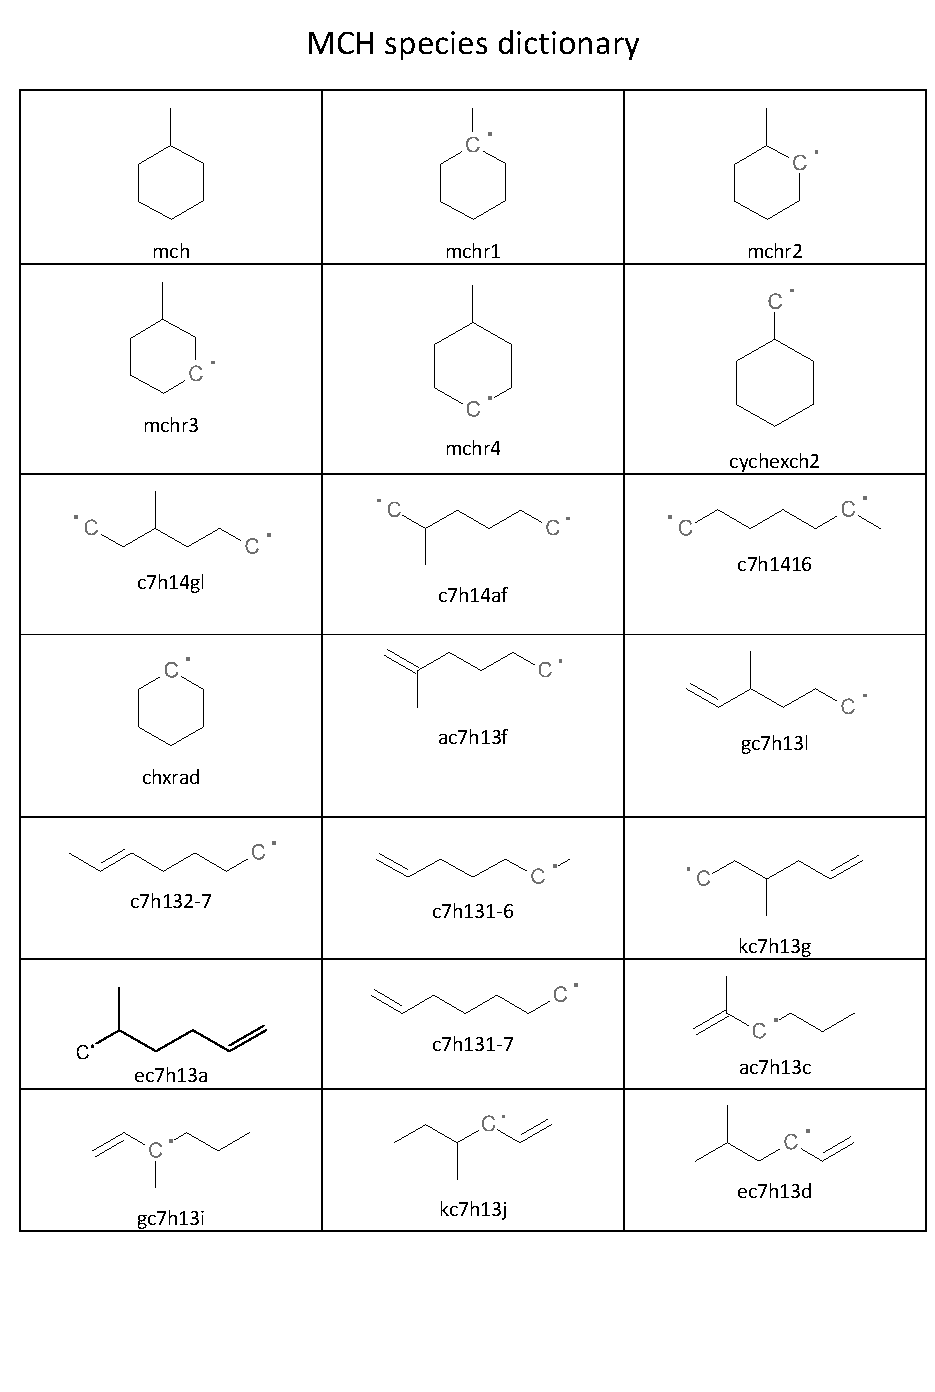
\includepdf[scale=0.85,pages={-},pagecommand={}]{includes/mch-species}

%Fast Sampling System
\chapter{Fast Sampling System}
\label{app:fast-sampling-system}

\subfile{chapters/B-Fast-Sampling-System}

%CanSen documentation
\chapter{CanSen}
\label{app:cansen}
CanSen is a Python script that I wrote to simplify the transition from
Senkin-style, input-file-based usage to the Cantera-style script-based usage.
The documentation included below is also available on the Web at
\url{http://bryanwweber.github.io/CanSen/html/index.html}.

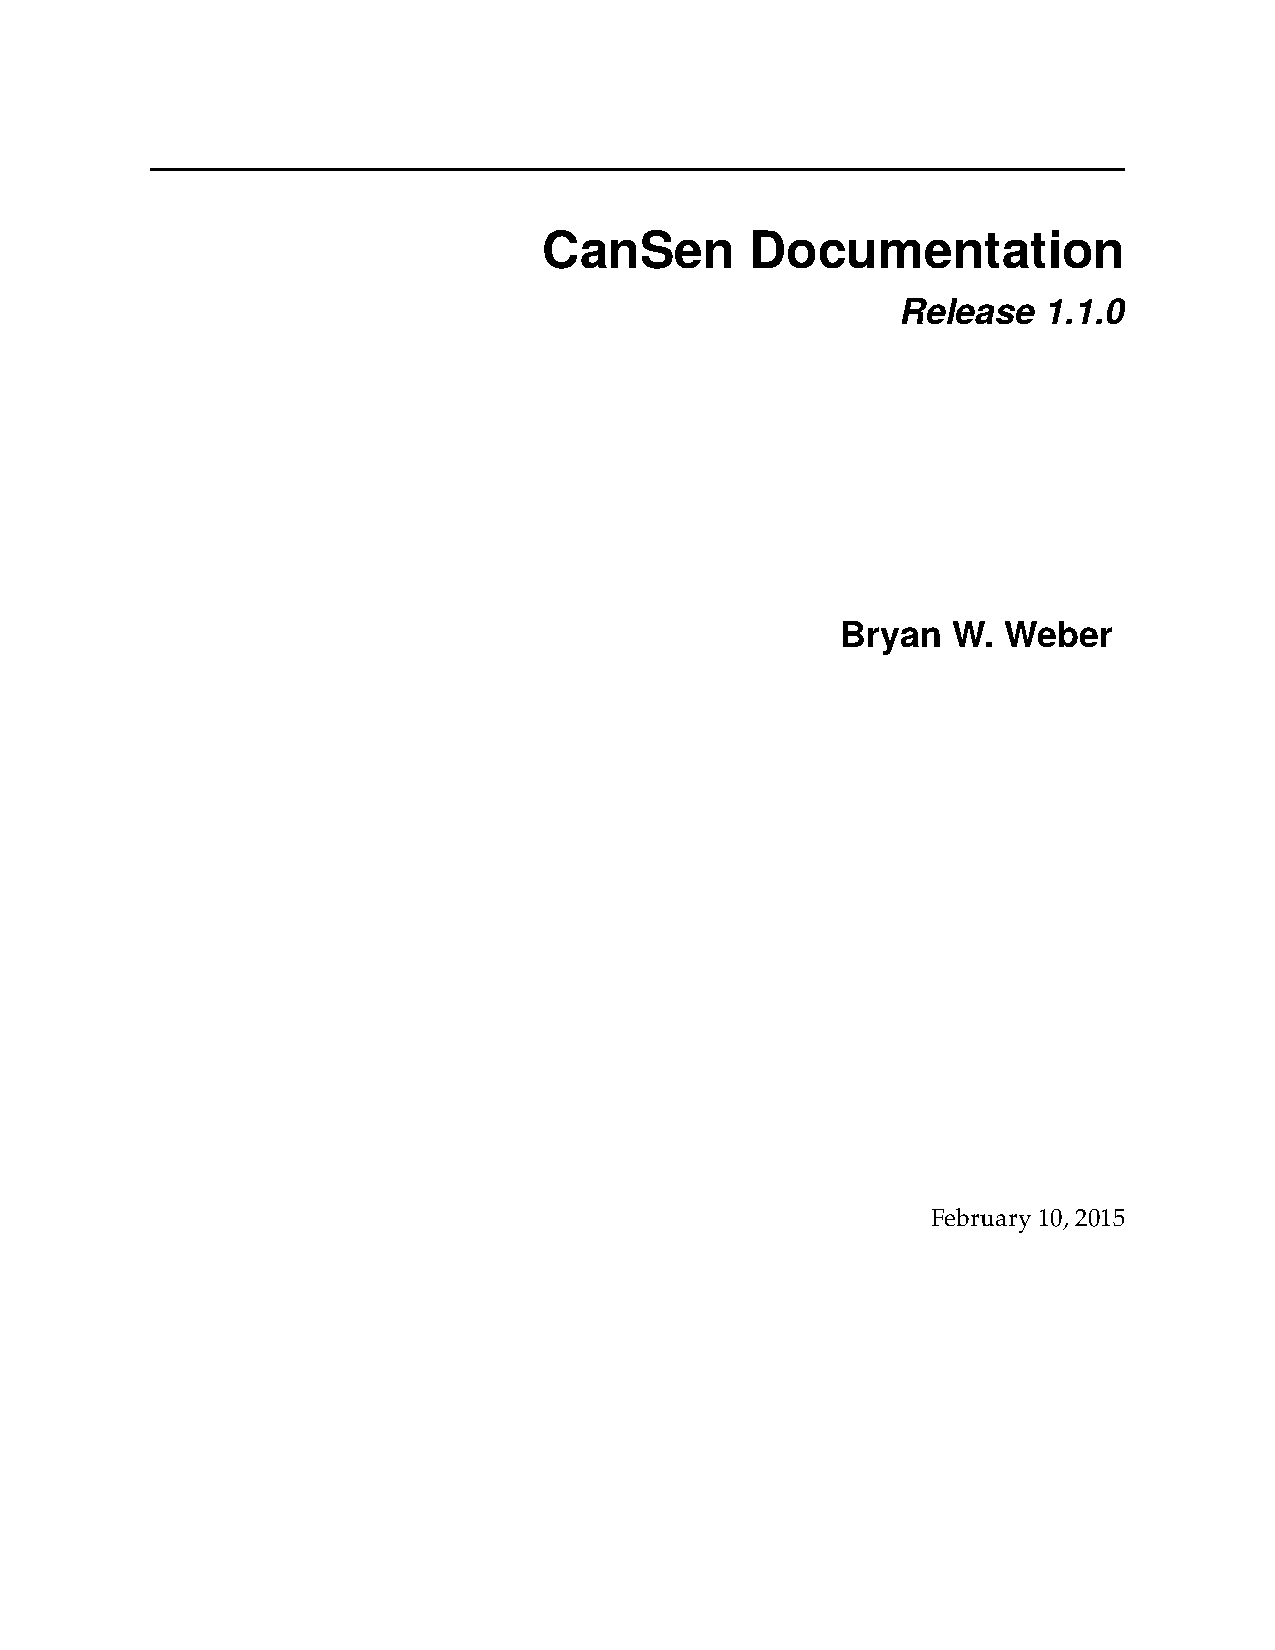
\includepdf[pages={-},pagecommand={}]{includes/CanSen}

%Pysens code
\chapter{pysens}
\label{app:pysens}
This appendix contains the code for `pysens`. `pysens` is a Python wrapper
for sensitivity analysis in CHEMKIN-Pro. This program runs a brute
force, one-at-a-time sensitivity analysis of the ignition delay for a
given mechanism. It was used to conduct the sensitivity analyses in
\cref{chap:peoh,chap:mch}

\blankline


\begin{singlespace}
{\setlength{\parindent}{0pt}
\DefineShortVerb[commandchars=\\\{\}]{\`}
{\large \textbf{Usage:}}

Download the repository by using Git: 

`git clone git://github.com/bryanwweber/pysens.git`

No other compilation is necessary. Python 3 is required.
The runtime behavior of the script is configured by setting options in
the `pysens.conf` file. A sample `pysens.conf` is included in the
distribution and reproduced below.

The script can be run on Linux either by setting the executable bit
and executing the program from the shell e.g.\\
`./run_sens.py`\\
or by calling\\
`python3 run_sens.py`.\\
On Windows, it should be run by\\
`py run_sens.py`\\
Note: I haven't tested this on Windows

\blankline

{\large `pysens.conf` \textbf{options:}}

The `pysens.conf` file must either have `[DEFAULT]` on the first line,
or one of the following options. No other text is supported on the first
line. If options are given that aren't specified below, they will be
ignored.

The options can be specified by:

`option = value or option : value`

The following options are available:

\begin{Verbatim}
reactions - The set of reactions to be analyzed. Can be one of:

all - use all of the reactions in the mechanism
comma-separated list (e.g. 1,2,3) - use the specified reactions
colon-separated values - specify a range of reactions with either start:stop or
                         start:interval:stop syntax. If stop is not given, it
                         defaults to the number of reactions in the mechanism.
                         Thus, all and 1: are equivalent. end is a
                         synonym for the number of reactions. E.g. 1:10 or
                         1:2:10 or 1:2: or 1:2:end

mech input file - The mechanism to be analyzed.

thermo input file - Optional if the thermo information
                    is specified in the mech input file.

outputfile - The base name of the output file. The full
             output file name will be set by concatenating
             outputfile + rfactor + sim input file.

factors - The multiplication factors to be considered.
          Multiple multiplication factors should be
          separated by commas.

sim input files - Valid CHEMKIN-Pro input files for the
                  test cases desired.

chemkin root - The root directory of the CHEMKIN-Pro
               install. Accepts shell variables, including
               those set by the CHEMKIN setup script
               that should run at logon.
\end{Verbatim}

{\large \textbf{Sample} `pysens.conf` \textbf{file:}}
\VerbatimInput{includes/pysens.conf}

The following is the code that makes up this script.

\cleardoublepage

{\Large `run\_sens.py`, the main driver script}
\begin{Verbatim}[commandchars=\\\{\},fontsize=\small,numbers=left,firstnumber=1,stepnumber=2,firstline=2]

\PY{c}{\PYZsh{}! /usr/bin/python3 \PYZhy{}u}

\PY{c}{\PYZsh{} System imports}
\PY{k+kn}{import} \PY{n+nn}{re}
\PY{k+kn}{import} \PY{n+nn}{os}
\PY{k+kn}{import} \PY{n+nn}{subprocess}
\PY{k+kn}{import} \PY{n+nn}{shutil}
\PY{k+kn}{import} \PY{n+nn}{sys}
\PY{k+kn}{from} \PY{n+nn}{itertools} \PY{k+kn}{import} \PY{n}{product}
\PY{k+kn}{from} \PY{n+nn}{decimal} \PY{k+kn}{import} \PY{o}{*}

\PY{c}{\PYZsh{} Local imports}
\PY{k+kn}{from} \PY{n+nn}{mechinterp} \PY{k+kn}{import} \PY{n}{mechinterp}
\PY{k+kn}{from} \PY{n+nn}{sens\PYZus{}helper} \PY{k+kn}{import} \PY{o}{*}

\PY{k}{def} \PY{n+nf}{main}\PY{p}{(}\PY{p}{)}\PY{p}{:}
    \PY{c}{\PYZsh{} Read the configuration file.}
    \PY{n}{config} \PY{o}{=} \PY{n}{NoSectionConfigParser}\PY{p}{(}\PY{p}{)}
    \PY{n}{config}\PY{o}{.}\PY{n}{read}\PY{p}{(}\PY{l+s}{\PYZsq{}}\PY{l+s}{pysens.conf}\PY{l+s}{\PYZsq{}}\PY{p}{)}
    \PY{n}{default} \PY{o}{=} \PY{n}{config}\PY{p}{[}\PY{l+s}{\PYZsq{}}\PY{l+s}{DEFAULT}\PY{l+s}{\PYZsq{}}\PY{p}{]}

    \PY{c}{\PYZsh{} Set the location of the CHEMKIN executable files. Expand any shell}
    \PY{c}{\PYZsh{} variables in the input.}
    \PY{n}{reactiondir} \PY{o}{=} \PY{n}{default}\PY{p}{[}\PY{l+s}{\PYZsq{}}\PY{l+s}{chemkin root}\PY{l+s}{\PYZsq{}}\PY{p}{]}
    \PY{k}{if} \PY{l+s}{\PYZsq{}}\PY{l+s}{\PYZdl{}}\PY{l+s}{\PYZsq{}} \PY{o+ow}{in} \PY{n}{reactiondir}\PY{p}{:}
        \PY{n}{reactiondir} \PY{o}{=} \PY{n}{os}\PY{o}{.}\PY{n}{path}\PY{o}{.}\PY{n}{expandvars}\PY{p}{(}\PY{n}{reactiondir}\PY{p}{)}
        \PY{k}{if} \PY{n}{os}\PY{o}{.}\PY{n}{path}\PY{o}{.}\PY{n}{isdir}\PY{p}{(}\PY{n}{reactiondir}\PY{p}{)}\PY{p}{:}
            \PY{n}{reactor} \PY{o}{=} \PY{n}{os}\PY{o}{.}\PY{n}{path}\PY{o}{.}\PY{n}{join}\PY{p}{(}\PY{n}{reactiondir}\PY{p}{,}\PY{l+s}{\PYZsq{}}\PY{l+s}{bin}\PY{l+s}{\PYZsq{}}\PY{p}{,}\PY{l+s}{\PYZsq{}}\PY{l+s}{CKReactorGenericClosed}\PY{l+s}{\PYZsq{}}\PY{p}{)}
            \PY{n}{ckinterp} \PY{o}{=} \PY{n}{os}\PY{o}{.}\PY{n}{path}\PY{o}{.}\PY{n}{join}\PY{p}{(}\PY{n}{reactiondir}\PY{p}{,}\PY{l+s}{\PYZsq{}}\PY{l+s}{bin}\PY{l+s}{\PYZsq{}}\PY{p}{,}\PY{l+s}{\PYZsq{}}\PY{l+s}{chem}\PY{l+s}{\PYZsq{}}\PY{p}{)}
            \PY{k}{if} \PY{o+ow}{not} \PY{n}{os}\PY{o}{.}\PY{n}{path}\PY{o}{.}\PY{n}{isfile}\PY{p}{(}\PY{n}{reactor}\PY{p}{)} \PY{o+ow}{or} \PY{o+ow}{not} \PY{n}{os}\PY{o}{.}\PY{n}{path}\PY{o}{.}\PY{n}{isfile}\PY{p}{(}\PY{n}{ckinterp}\PY{p}{)}\PY{p}{:}
                \PY{k}{print}\PY{p}{(}\PY{l+s}{\PYZdq{}}\PY{l+s}{Error: The reactor and CHEMKIN interpreter must }\PY{l+s}{\PYZdq{}}
                      \PY{l+s}{\PYZdq{}}\PY{l+s}{exist at CHEMKIN\PYZus{}ROOT/bin/}\PY{l+s}{\PYZdq{}}\PY{p}{)}
                \PY{n}{sys}\PY{o}{.}\PY{n}{exit}\PY{p}{(}\PY{l+m+mi}{1}\PY{p}{)}
        \PY{k}{else}\PY{p}{:}
            \PY{k}{print}\PY{p}{(}\PY{l+s}{\PYZdq{}}\PY{l+s}{Error: The proper path to the CHEMKIN root }\PY{l+s}{\PYZdq{}}
                  \PY{l+s}{\PYZdq{}}\PY{l+s}{directory must be specified}\PY{l+s}{\PYZdq{}}\PY{p}{)}
            \PY{n}{sys}\PY{o}{.}\PY{n}{exit}\PY{p}{(}\PY{l+m+mi}{1}\PY{p}{)}

    \PY{c}{\PYZsh{} Set the mechanism to be used.}
    \PY{k}{if} \PY{p}{(}\PY{l+s}{\PYZsq{}}\PY{l+s}{mech input file}\PY{l+s}{\PYZsq{}} \PY{o+ow}{in} \PY{n}{default} \PY{o+ow}{and}
            \PY{n}{os}\PY{o}{.}\PY{n}{path}\PY{o}{.}\PY{n}{isfile}\PY{p}{(}\PY{n}{default}\PY{p}{[}\PY{l+s}{\PYZsq{}}\PY{l+s}{mech input file}\PY{l+s}{\PYZsq{}}\PY{p}{]}\PY{p}{)}\PY{p}{)}\PY{p}{:}
        \PY{n}{inputfilename} \PY{o}{=} \PY{n}{default}\PY{p}{[}\PY{l+s}{\PYZsq{}}\PY{l+s}{mech input file}\PY{l+s}{\PYZsq{}}\PY{p}{]}
    \PY{k}{else}\PY{p}{:}
        \PY{k}{print}\PY{p}{(}\PY{l+s}{\PYZdq{}}\PY{l+s}{Error: the mechanism file must be specified in the }\PY{l+s}{\PYZdq{}}
              \PY{l+s}{\PYZdq{}}\PY{l+s}{configuration file, and it must exist}\PY{l+s}{\PYZdq{}}\PY{p}{)}
        \PY{n}{sys}\PY{o}{.}\PY{n}{exit}\PY{p}{(}\PY{l+m+mi}{1}\PY{p}{)}

    \PY{c}{\PYZsh{} Set the simulation input file to be used.}
    \PY{k}{if} \PY{l+s}{\PYZsq{}}\PY{l+s}{sim input files}\PY{l+s}{\PYZsq{}} \PY{o+ow}{in} \PY{n}{default}\PY{p}{:}
        \PY{n}{siminputfiles} \PY{o}{=} \PY{p}{[}\PY{n}{x}\PY{o}{.}\PY{n}{strip}\PY{p}{(}\PY{p}{)} \PY{k}{for} \PY{n}{x} \PY{o+ow}{in}
                         \PY{n}{default}\PY{p}{[}\PY{l+s}{\PYZsq{}}\PY{l+s}{sim input files}\PY{l+s}{\PYZsq{}}\PY{p}{]}\PY{o}{.}\PY{n}{split}\PY{p}{(}\PY{l+s}{\PYZsq{}}\PY{l+s}{,}\PY{l+s}{\PYZsq{}}\PY{p}{)}
                         \PY{p}{]}
        \PY{k}{for} \PY{n}{fname} \PY{o+ow}{in} \PY{n}{siminputfiles}\PY{p}{:}
            \PY{k}{if} \PY{o+ow}{not} \PY{n}{os}\PY{o}{.}\PY{n}{path}\PY{o}{.}\PY{n}{isfile}\PY{p}{(}\PY{n}{fname}\PY{p}{)}\PY{p}{:}
                \PY{k}{print}\PY{p}{(}\PY{l+s}{\PYZdq{}}\PY{l+s}{Error: the specified input file \PYZob{}\PYZcb{} does not }\PY{l+s}{\PYZdq{}}
                      \PY{l+s}{\PYZdq{}}\PY{l+s}{exist}\PY{l+s}{\PYZdq{}}\PY{o}{.}\PY{n}{format}\PY{p}{(}\PY{n}{fname}\PY{p}{)}\PY{p}{)}
                \PY{n}{sys}\PY{o}{.}\PY{n}{exit}\PY{p}{(}\PY{l+m+mi}{1}\PY{p}{)}
    \PY{k}{else}\PY{p}{:}
        \PY{k}{print}\PY{p}{(}\PY{l+s}{\PYZdq{}}\PY{l+s}{Error: the simulation input file must be specified in }\PY{l+s}{\PYZdq{}}
              \PY{l+s}{\PYZdq{}}\PY{l+s}{the configuration file}\PY{l+s}{\PYZdq{}}\PY{p}{)}
        \PY{n}{sys}\PY{o}{.}\PY{n}{exit}\PY{p}{(}\PY{l+m+mi}{1}\PY{p}{)}

    \PY{c}{\PYZsh{} Set the multiplication factors to be used.}
    \PY{k}{if} \PY{l+s}{\PYZsq{}}\PY{l+s}{factors}\PY{l+s}{\PYZsq{}} \PY{o+ow}{in} \PY{n}{default}\PY{p}{:}
        \PY{n}{multfactors} \PY{o}{=} \PY{p}{[}\PY{n}{x}\PY{o}{.}\PY{n}{strip} \PY{k}{for} \PY{n}{x} \PY{o+ow}{in} \PY{n}{default}\PY{p}{[}\PY{l+s}{\PYZsq{}}\PY{l+s}{factors}\PY{l+s}{\PYZsq{}}\PY{p}{]}\PY{o}{.}\PY{n}{split}\PY{p}{(}\PY{l+s}{\PYZsq{}}\PY{l+s}{,}\PY{l+s}{\PYZsq{}}\PY{p}{)}\PY{p}{]}
    \PY{k}{else}\PY{p}{:}
        \PY{k}{print}\PY{p}{(}\PY{l+s}{\PYZdq{}}\PY{l+s}{Error: at least one multiplication factor must be }\PY{l+s}{\PYZdq{}}
              \PY{l+s}{\PYZdq{}}\PY{l+s}{specified in the configuration file}\PY{l+s}{\PYZdq{}}\PY{p}{)}
        \PY{n}{sys}\PY{o}{.}\PY{n}{exit}\PY{p}{(}\PY{l+m+mi}{1}\PY{p}{)}

    \PY{c}{\PYZsh{}Set the base of the csv output file name.}
    \PY{k}{if} \PY{l+s}{\PYZsq{}}\PY{l+s}{outputfile}\PY{l+s}{\PYZsq{}} \PY{o+ow}{in} \PY{n}{default}\PY{p}{:}
        \PY{n}{sensfilenamebase} \PY{o}{=} \PY{n}{default}\PY{p}{[}\PY{l+s}{\PYZsq{}}\PY{l+s}{outputfile}\PY{l+s}{\PYZsq{}}\PY{p}{]}
    \PY{k}{else}\PY{p}{:}
        \PY{k}{print}\PY{p}{(}\PY{l+s}{\PYZdq{}}\PY{l+s}{Error: the base of the csv output filename must be }\PY{l+s}{\PYZdq{}}
              \PY{l+s}{\PYZdq{}}\PY{l+s}{specified in the configuration file}\PY{l+s}{\PYZdq{}}\PY{p}{)}
        \PY{n}{sys}\PY{o}{.}\PY{n}{exit}\PY{p}{(}\PY{l+m+mi}{1}\PY{p}{)}

    \PY{c}{\PYZsh{} Compile the required regular expressions}
    \PY{n}{commentmatch} \PY{o}{=} \PY{n}{re}\PY{o}{.}\PY{n}{compile}\PY{p}{(}\PY{l+s}{r\PYZsq{}}\PY{l+s}{\PYZca{}}\PY{l+s}{\PYZbs{}}\PY{l+s}{!}\PY{l+s}{\PYZsq{}}\PY{p}{)}
    \PY{n}{newlinematch} \PY{o}{=} \PY{n}{re}\PY{o}{.}\PY{n}{compile}\PY{p}{(}\PY{l+s}{r\PYZsq{}}\PY{l+s}{\PYZca{}}\PY{l+s}{\PYZbs{}}\PY{l+s}{n}\PY{l+s}{\PYZsq{}}\PY{p}{)}

    \PY{c}{\PYZsh{} The following regular expressions match the keywords we expect to}
    \PY{c}{\PYZsh{}see. The `(?i)` indicates case insensitive. For certain keywords,}
    \PY{c}{\PYZsh{} we want to match the keyword even if there is space at the}
    \PY{c}{\PYZsh{} beginning of the line; these keywords have `\PYZca{}[\PYZbs{}s]*`.}
    \PY{n}{lowmatch} \PY{o}{=} \PY{n}{re}\PY{o}{.}\PY{n}{compile}\PY{p}{(}\PY{l+s}{r\PYZsq{}}\PY{l+s}{(?i)\PYZca{}[}\PY{l+s}{\PYZbs{}}\PY{l+s}{s]*LOW}\PY{l+s}{\PYZsq{}}\PY{p}{)}
    \PY{n}{highmatch} \PY{o}{=} \PY{n}{re}\PY{o}{.}\PY{n}{compile}\PY{p}{(}\PY{l+s}{r\PYZsq{}}\PY{l+s}{(?i)\PYZca{}[}\PY{l+s}{\PYZbs{}}\PY{l+s}{s]*HIGH}\PY{l+s}{\PYZsq{}}\PY{p}{)}
    \PY{n}{dupmatch} \PY{o}{=} \PY{n}{re}\PY{o}{.}\PY{n}{compile}\PY{p}{(}\PY{l+s}{r\PYZsq{}}\PY{l+s}{(?i)}\PY{l+s}{\PYZbs{}}\PY{l+s}{bDUP}\PY{l+s}{\PYZbs{}}\PY{l+s}{b|}\PY{l+s}{\PYZbs{}}\PY{l+s}{bDUPLICATE}\PY{l+s}{\PYZbs{}}\PY{l+s}{b}\PY{l+s}{\PYZsq{}}\PY{p}{)}
    \PY{n}{endmatch} \PY{o}{=} \PY{n}{re}\PY{o}{.}\PY{n}{compile}\PY{p}{(}\PY{l+s}{r\PYZsq{}}\PY{l+s}{(?i)\PYZca{}END}\PY{l+s}{\PYZsq{}}\PY{p}{)}
    \PY{n}{revmatch} \PY{o}{=} \PY{n}{re}\PY{o}{.}\PY{n}{compile}\PY{p}{(}\PY{l+s}{r\PYZsq{}}\PY{l+s}{(?i)\PYZca{}[}\PY{l+s}{\PYZbs{}}\PY{l+s}{s]*REV}\PY{l+s}{\PYZsq{}}\PY{p}{)}
    \PY{n}{plogmatch} \PY{o}{=} \PY{n}{re}\PY{o}{.}\PY{n}{compile}\PY{p}{(}\PY{l+s}{r\PYZsq{}}\PY{l+s}{(?i)\PYZca{}[}\PY{l+s}{\PYZbs{}}\PY{l+s}{s]*PLOG}\PY{l+s}{\PYZsq{}}\PY{p}{)}
    \PY{n}{Amatch} \PY{o}{=} \PY{n}{re}\PY{o}{.}\PY{n}{compile}\PY{p}{(}\PY{l+s}{r\PYZsq{}}\PY{l+s}{((?\PYZlt{}![}\PY{l+s}{\PYZbs{}}\PY{l+s}{w}\PY{l+s}{\PYZbs{}}\PY{l+s}{\PYZhy{}])([\PYZhy{}+]?[0\PYZhy{}9]+(}\PY{l+s}{\PYZbs{}}\PY{l+s}{.[0\PYZhy{}9]+)?}\PY{l+s}{\PYZsq{}}
                        \PY{l+s}{\PYZsq{}}\PY{l+s}{([eE][\PYZhy{}+]?[0\PYZhy{}9]+)?)(?!}\PY{l+s}{\PYZbs{}}\PY{l+s}{w))}\PY{l+s}{\PYZsq{}}
                        \PY{p}{)}
    \PY{n}{reacmatch} \PY{o}{=} \PY{n}{re}\PY{o}{.}\PY{n}{compile}\PY{p}{(}\PY{l+s}{r\PYZsq{}}\PY{l+s}{((\PYZca{}|\PYZca{}[}\PY{l+s}{\PYZbs{}}\PY{l+s}{s]+)[}\PY{l+s}{\PYZbs{}}\PY{l+s}{s}\PY{l+s}{\PYZbs{}}\PY{l+s}{w}\PY{l+s}{\PYZbs{}}\PY{l+s}{d()+=\PYZlt{}\PYZgt{}}\PY{l+s}{\PYZbs{}}\PY{l+s}{\PYZhy{} *.]+?(?=}\PY{l+s}{\PYZbs{}}\PY{l+s}{s}\PY{l+s}{\PYZbs{}}\PY{l+s}{d))}\PY{l+s}{\PYZsq{}}\PY{p}{)}

    \PY{c}{\PYZsh{} Open, read, and close the input file. The lines of the input file}
    \PY{c}{\PYZsh{} are stored in the list `lines`.}
    \PY{k}{try}\PY{p}{:}
        \PY{k}{with} \PY{n+nb}{open}\PY{p}{(}\PY{n}{inputfilename}\PY{p}{,} \PY{l+s}{\PYZsq{}}\PY{l+s}{rt}\PY{l+s}{\PYZsq{}}\PY{p}{)} \PY{k}{as} \PY{n}{inputfile}\PY{p}{:}
            \PY{n}{lines} \PY{o}{=} \PY{n}{inputfile}\PY{o}{.}\PY{n}{readlines}\PY{p}{(}\PY{p}{)}
    \PY{k}{except} \PY{n+ne}{UnicodeDecodeError}\PY{p}{:}
        \PY{k}{with} \PY{n+nb}{open}\PY{p}{(}\PY{n}{inputfilename}\PY{p}{,}\PY{l+s}{\PYZsq{}}\PY{l+s}{rt}\PY{l+s}{\PYZsq{}}\PY{p}{,} \PY{n}{encoding}\PY{o}{=}\PY{l+s}{\PYZsq{}}\PY{l+s}{latin\PYZhy{}1}\PY{l+s}{\PYZsq{}}\PY{p}{)} \PY{k}{as} \PY{n}{inputfile}\PY{p}{:}
            \PY{n}{lines} \PY{o}{=} \PY{n}{inputfile}\PY{o}{.}\PY{n}{readlines}\PY{p}{(}\PY{p}{)}
    \PY{k}{else}\PY{p}{:}
        \PY{k}{print}\PY{p}{(}\PY{l+s}{\PYZdq{}}\PY{l+s}{Error: I can}\PY{l+s}{\PYZsq{}}\PY{l+s}{t decode the input file. Try saving it }\PY{l+s}{\PYZdq{}}
              \PY{l+s}{\PYZdq{}}\PY{l+s}{as UTF\PYZhy{}8}\PY{l+s}{\PYZdq{}}\PY{p}{)}
        \PY{n}{sys}\PY{o}{.}\PY{n}{exit}\PY{p}{(}\PY{l+m+mi}{1}\PY{p}{)}

    \PY{c}{\PYZsh{} Call the mechanism interpreter module. The mechinterp function}
    \PY{c}{\PYZsh{} returns a tuple of lists plus a boolean. The lists contain the}
    \PY{c}{\PYZsh{} line numbers in the input file of the reactions, the lines between}
    \PY{c}{\PYZsh{} each reaction, and whether a reaction has auxiliary information.}
    \PY{c}{\PYZsh{} The boolean checks whether the thermo data is available in the}
    \PY{c}{\PYZsh{} chemistry file or if it should be taken from a separate file.}
    \PY{c}{\PYZsh{} These are stored, respectively, in `reacLines`, `searchLines`,}
    \PY{c}{\PYZsh{} `extraInfo` and `thermInChem`.}
    \PY{n}{reacLines}\PY{p}{,} \PY{n}{searchLines}\PY{p}{,} \PY{n}{extraInfo}\PY{p}{,} \PY{n}{thermInChem}\PY{p}{,} \PY{o}{=} \PY{n}{mechinterp}\PY{p}{(}\PY{n}{lines}\PY{p}{)}

    \PY{c}{\PYZsh{} Set the thermo file, if necessary.}
    \PY{k}{if} \PY{p}{(}\PY{o+ow}{not} \PY{n}{thermInChem} \PY{o+ow}{and} \PY{l+s}{\PYZsq{}}\PY{l+s}{thermo input file}\PY{l+s}{\PYZsq{}} \PY{o+ow}{in} \PY{n}{default} \PY{o+ow}{and}
            \PY{n}{os}\PY{o}{.}\PY{n}{path}\PY{o}{.}\PY{n}{isfile}\PY{p}{(}\PY{n}{default}\PY{p}{[}\PY{l+s}{\PYZsq{}}\PY{l+s}{thermo input file}\PY{l+s}{\PYZsq{}}\PY{p}{]}\PY{p}{)}\PY{p}{)}\PY{p}{:}
        \PY{n}{thermfilename} \PY{o}{=} \PY{n}{default}\PY{p}{[}\PY{l+s}{\PYZsq{}}\PY{l+s}{thermo input file}\PY{l+s}{\PYZsq{}}\PY{p}{]}
    \PY{k}{elif} \PY{p}{(}\PY{o+ow}{not} \PY{n}{thermInChem} \PY{o+ow}{and} \PY{p}{(}\PY{o+ow}{not} \PY{l+s}{\PYZsq{}}\PY{l+s}{thermo input file}\PY{l+s}{\PYZsq{}} \PY{o+ow}{in} \PY{n}{default} \PY{o+ow}{or} \PY{o+ow}{not}
            \PY{n}{os}\PY{o}{.}\PY{n}{path}\PY{o}{.}\PY{n}{isfile}\PY{p}{(}\PY{n}{default}\PY{p}{[}\PY{l+s}{\PYZsq{}}\PY{l+s}{thermo input file}\PY{l+s}{\PYZsq{}}\PY{p}{]}\PY{p}{)}\PY{p}{)}\PY{p}{)}\PY{p}{:}
        \PY{k}{print}\PY{p}{(}\PY{l+s}{\PYZdq{}}\PY{l+s}{Error: the thermo file must be specified in the }\PY{l+s}{\PYZdq{}}
              \PY{l+s}{\PYZdq{}}\PY{l+s}{configuration file, and it must exist}\PY{l+s}{\PYZdq{}}\PY{p}{)}
        \PY{n}{sys}\PY{o}{.}\PY{n}{exit}\PY{p}{(}\PY{l+m+mi}{1}\PY{p}{)}

    \PY{c}{\PYZsh{} Set the reactions we want to work with.}
    \PY{n}{numRxns} \PY{o}{=} \PY{n+nb}{len}\PY{p}{(}\PY{n}{reacLines}\PY{p}{)}\PY{o}{\PYZhy{}}\PY{l+m+mi}{1}
    \PY{k}{if} \PY{o+ow}{not} \PY{l+s}{\PYZsq{}}\PY{l+s}{reactions}\PY{l+s}{\PYZsq{}} \PY{o+ow}{in} \PY{n}{default}\PY{p}{:}
        \PY{k}{print}\PY{p}{(}\PY{l+s}{\PYZdq{}}\PY{l+s}{Error: the reactions to study must be specified in the }\PY{l+s}{\PYZdq{}}
              \PY{l+s}{\PYZdq{}}\PY{l+s}{configuration file}\PY{l+s}{\PYZdq{}}\PY{p}{)}
        \PY{n}{sys}\PY{o}{.}\PY{n}{exit}\PY{p}{(}\PY{l+m+mi}{1}\PY{p}{)}
    \PY{k}{else}\PY{p}{:}
        \PY{n}{wantrxns} \PY{o}{=} \PY{n}{default}\PY{p}{[}\PY{l+s}{\PYZsq{}}\PY{l+s}{reactions}\PY{l+s}{\PYZsq{}}\PY{p}{]}

    \PY{k}{if} \PY{n}{wantrxns} \PY{o}{==} \PY{n+nb}{all}\PY{p}{:}
        \PY{n}{wantreactions} \PY{o}{=} \PY{p}{[}\PY{n}{x} \PY{o}{+} \PY{l+m+mi}{1} \PY{k}{for} \PY{n}{x} \PY{o+ow}{in} \PY{n+nb}{range}\PY{p}{(}\PY{n}{numRxns}\PY{p}{)}\PY{p}{]}
        \PY{k}{print}\PY{p}{(}\PY{l+s}{\PYZdq{}}\PY{l+s}{All \PYZob{}\PYZcb{} reactions are considered in these }\PY{l+s}{\PYZdq{}}
              \PY{l+s}{\PYZdq{}}\PY{l+s}{analyses}\PY{l+s}{\PYZdq{}}\PY{o}{.}\PY{n}{format}\PY{p}{(}\PY{n}{numRxns}\PY{p}{)}\PY{p}{)}
    \PY{k}{elif} \PY{l+s}{\PYZsq{}}\PY{l+s}{,}\PY{l+s}{\PYZsq{}} \PY{o+ow}{in} \PY{n}{wantrxns} \PY{o+ow}{and} \PY{l+s}{\PYZsq{}}\PY{l+s}{:}\PY{l+s}{\PYZsq{}} \PY{o+ow}{in} \PY{n}{wantrxns}\PY{p}{:}
        \PY{k}{print}\PY{p}{(}\PY{l+s}{\PYZdq{}}\PY{l+s}{Error: use one of commas or colons to separate the wanted }\PY{l+s}{\PYZdq{}}
              \PY{l+s}{\PYZdq{}}\PY{l+s}{reactions}\PY{l+s}{\PYZdq{}}\PY{p}{)}
        \PY{n}{sys}\PY{o}{.}\PY{n}{exit}\PY{p}{(}\PY{l+m+mi}{1}\PY{p}{)}
    \PY{k}{elif} \PY{l+s}{\PYZsq{}}\PY{l+s}{,}\PY{l+s}{\PYZsq{}} \PY{o+ow}{in} \PY{n}{wantrxns}\PY{p}{:}
        \PY{n}{wantreactions} \PY{o}{=} \PY{p}{[}\PY{n+nb}{int}\PY{p}{(}\PY{n}{number}\PY{p}{)} \PY{k}{for} \PY{n}{number} \PY{o+ow}{in} \PY{n}{wantrxns}\PY{o}{.}\PY{n}{split}\PY{p}{(}\PY{l+s}{\PYZsq{}}\PY{l+s}{,}\PY{l+s}{\PYZsq{}}\PY{p}{)} \PY{k}{if}
            \PY{n}{number}\PY{p}{]}
        \PY{k}{print}\PY{p}{(}\PY{l+s}{\PYZdq{}}\PY{l+s}{The reactions considered in these analyses are }\PY{l+s}{\PYZdq{}}
              \PY{l+s}{\PYZdq{}}\PY{l+s}{\PYZob{}\PYZcb{}}\PY{l+s}{\PYZdq{}}\PY{o}{.}\PY{n}{format}\PY{p}{(}\PY{n}{wantreactions}\PY{p}{)}\PY{p}{)}
    \PY{k}{elif} \PY{l+s}{\PYZsq{}}\PY{l+s}{:}\PY{l+s}{\PYZsq{}} \PY{o+ow}{in} \PY{n}{wantrxns}\PY{p}{:}
        \PY{k}{if} \PY{n}{wantrxns}\PY{o}{.}\PY{n}{endswith}\PY{p}{(}\PY{l+s}{\PYZsq{}}\PY{l+s}{:}\PY{l+s}{\PYZsq{}}\PY{p}{)} \PY{o+ow}{or} \PY{n}{wantrxns}\PY{o}{.}\PY{n}{endswith}\PY{p}{(}\PY{l+s}{\PYZsq{}}\PY{l+s}{end}\PY{l+s}{\PYZsq{}}\PY{p}{)}\PY{p}{:}
            \PY{n}{spl} \PY{o}{=} \PY{n+nb}{list}\PY{p}{(}\PY{n+nb}{map}\PY{p}{(}\PY{n+nb}{int}\PY{p}{,} \PY{n}{wantrxns}\PY{o}{.}\PY{n}{split}\PY{p}{(}\PY{l+s}{\PYZsq{}}\PY{l+s}{:}\PY{l+s}{\PYZsq{}}\PY{p}{)}\PY{p}{[}\PY{p}{:}\PY{o}{\PYZhy{}}\PY{l+m+mi}{1}\PY{p}{]}\PY{p}{)}\PY{p}{)}
            \PY{n}{spl}\PY{o}{.}\PY{n}{append}\PY{p}{(}\PY{n}{numRxns}\PY{p}{)}
        \PY{k}{else}\PY{p}{:}
            \PY{n}{spl} \PY{o}{=} \PY{n+nb}{list}\PY{p}{(}\PY{n+nb}{map}\PY{p}{(}\PY{n+nb}{int}\PY{p}{,} \PY{n}{wantrxns}\PY{o}{.}\PY{n}{split}\PY{p}{(}\PY{l+s}{\PYZsq{}}\PY{l+s}{:}\PY{l+s}{\PYZsq{}}\PY{p}{)}\PY{p}{)}\PY{p}{)}

        \PY{k}{if} \PY{n+nb}{len}\PY{p}{(}\PY{n}{spl}\PY{p}{)} \PY{o}{==} \PY{l+m+mi}{2}\PY{p}{:}
            \PY{n}{wantreactions} \PY{o}{=} \PY{n+nb}{list}\PY{p}{(}\PY{n+nb}{range}\PY{p}{(}\PY{n}{spl}\PY{p}{[}\PY{l+m+mi}{0}\PY{p}{]}\PY{p}{,} \PY{n}{spl}\PY{p}{[}\PY{l+m+mi}{1}\PY{p}{]} \PY{o}{+} \PY{l+m+mi}{1}\PY{p}{)}\PY{p}{)}
        \PY{k}{elif} \PY{n+nb}{len}\PY{p}{(}\PY{n}{spl}\PY{p}{)} \PY{o}{==} \PY{l+m+mi}{3}\PY{p}{:}
            \PY{k}{if} \PY{n}{spl}\PY{p}{[}\PY{l+m+mi}{1}\PY{p}{]} \PY{o}{\PYZgt{}}\PY{o}{=} \PY{l+m+mi}{1}\PY{p}{:}
                \PY{n}{wantreactions} \PY{o}{=} \PY{n+nb}{list}\PY{p}{(}\PY{n+nb}{range}\PY{p}{(}\PY{n}{spl}\PY{p}{[}\PY{l+m+mi}{0}\PY{p}{]}\PY{p}{,} \PY{n}{spl}\PY{p}{[}\PY{l+m+mi}{2}\PY{p}{]} \PY{o}{+} \PY{l+m+mi}{1}\PY{p}{,} \PY{n}{spl}\PY{p}{[}\PY{l+m+mi}{1}\PY{p}{]}\PY{p}{)}\PY{p}{)}
            \PY{k}{else}\PY{p}{:}
                \PY{k}{print}\PY{p}{(}\PY{l+s}{\PYZdq{}}\PY{l+s}{Error: the interval in the reactions specification }\PY{l+s}{\PYZdq{}}
                      \PY{l+s}{\PYZdq{}}\PY{l+s}{must be \PYZgt{}= 1}\PY{l+s}{\PYZdq{}}\PY{p}{)}
                \PY{n}{sys}\PY{o}{.}\PY{n}{exit}\PY{p}{(}\PY{l+m+mi}{1}\PY{p}{)}
        \PY{k}{else}\PY{p}{:}
            \PY{k}{print}\PY{p}{(}\PY{l+s}{\PYZdq{}}\PY{l+s}{Error: Specify either start:stop or start:interval:stop }\PY{l+s}{\PYZdq{}}
                  \PY{l+s}{\PYZdq{}}\PY{l+s}{for reactions}\PY{l+s}{\PYZdq{}}\PY{p}{)}
            \PY{n}{sys}\PY{o}{.}\PY{n}{exit}\PY{p}{(}\PY{l+m+mi}{1}\PY{p}{)}
        \PY{k}{print}\PY{p}{(}\PY{l+s}{\PYZdq{}}\PY{l+s}{The reactions considered in these analyses are }\PY{l+s}{\PYZdq{}}
              \PY{l+s}{\PYZdq{}}\PY{l+s}{\PYZob{}\PYZcb{}}\PY{l+s}{\PYZdq{}}\PY{o}{.}\PY{n}{format}\PY{p}{(}\PY{n}{wantreactions}\PY{p}{)}\PY{p}{)}
    \PY{k}{else}\PY{p}{:}
        \PY{n}{wantreactions} \PY{o}{=} \PY{n+nb}{list}\PY{p}{(}\PY{n+nb}{int}\PY{p}{(}\PY{n}{wantrxns}\PY{p}{)}\PY{p}{)}
        \PY{k}{print}\PY{p}{(}\PY{l+s}{\PYZdq{}}\PY{l+s}{The reaction considered in these analyses is }\PY{l+s}{\PYZdq{}}
              \PY{l+s}{\PYZdq{}}\PY{l+s}{\PYZob{}\PYZcb{}}\PY{l+s}{\PYZdq{}}\PY{o}{.}\PY{n}{format}\PY{p}{(}\PY{n}{wantreactions}\PY{p}{)}\PY{p}{)}

    \PY{c}{\PYZsh{} Set filenames of simulation and output files.}
    \PY{n}{simoutputfile} \PY{o}{=} \PY{l+s}{\PYZsq{}}\PY{l+s}{test.out}\PY{l+s}{\PYZsq{}}
    \PY{n}{chemoutput} \PY{o}{=} \PY{l+s}{\PYZsq{}}\PY{l+s}{chem.out}\PY{l+s}{\PYZsq{}}
    \PY{n}{chemasc} \PY{o}{=} \PY{l+s}{\PYZsq{}}\PY{l+s}{chem.asc}\PY{l+s}{\PYZsq{}}
    \PY{n}{totalCases} \PY{o}{=} \PY{n+nb}{len}\PY{p}{(}\PY{n}{wantreactions}\PY{p}{)}\PY{o}{*}\PY{n+nb}{len}\PY{p}{(}\PY{n}{siminputfiles}\PY{p}{)}\PY{o}{*}\PY{n+nb}{len}\PY{p}{(}\PY{n}{multfactors}\PY{p}{)}
    \PY{k}{for} \PY{p}{(}\PY{n}{j}\PY{p}{,} \PY{p}{(}\PY{n}{inpfile}\PY{p}{,} \PY{n}{multfactor}\PY{p}{)} \PY{o+ow}{in}
            \PY{n+nb}{enumerate}\PY{p}{(}\PY{n}{product}\PY{p}{(}\PY{n}{siminputfiles}\PY{p}{,} \PY{n}{multfactors}\PY{p}{)}\PY{p}{)}\PY{p}{)}\PY{p}{:}
        \PY{n}{csvoutput} \PY{o}{=} \PY{p}{(}\PY{n}{sensfilenamebase} \PY{o}{+} \PY{l+s}{\PYZsq{}}\PY{l+s}{\PYZus{}}\PY{l+s}{\PYZsq{}} \PY{o}{+} \PY{n}{inpfile}\PY{o}{.}\PY{n}{strip}\PY{p}{(}\PY{l+s}{\PYZsq{}}\PY{l+s}{.inp}\PY{l+s}{\PYZsq{}}\PY{p}{)} \PY{o}{+} \PY{l+s}{\PYZsq{}}\PY{l+s}{\PYZus{}}\PY{l+s}{\PYZsq{}} \PY{o}{+}
            \PY{n}{multfactor} \PY{o}{+} \PY{l+s}{\PYZsq{}}\PY{l+s}{x.csv}\PY{l+s}{\PYZsq{}}\PY{p}{)}
        \PY{k}{with} \PY{n+nb}{open}\PY{p}{(}\PY{n}{csvoutput}\PY{p}{,} \PY{l+s}{\PYZsq{}}\PY{l+s}{at}\PY{l+s}{\PYZsq{}}\PY{p}{)} \PY{k}{as} \PY{n}{tignsens}\PY{p}{:}

            \PY{c}{\PYZsh{} Loop through the reaction numbers in `wantreaction`. `i`}
            \PY{c}{\PYZsh{} is the loop variable.}
            \PY{k}{for} \PY{n}{i}\PY{p}{,} \PY{n}{wantreaction} \PY{o+ow}{in} \PY{n+nb}{enumerate}\PY{p}{(}\PY{n}{wantreactions}\PY{p}{)}\PY{p}{:}

                \PY{c}{\PYZsh{} Python is zero\PYZhy{}based, so we have to subtract 1 from}
                \PY{c}{\PYZsh{} the numbers in `wantreaction` to properly find the}
                \PY{c}{\PYZsh{} index of the other lists}
                \PY{n}{rxnNum} \PY{o}{=} \PY{n}{wantreaction} \PY{o}{\PYZhy{}} \PY{l+m+mi}{1}

                \PY{c}{\PYZsh{} outLines is the list of lines to write to the chem.inp}
                \PY{c}{\PYZsh{} file to be run in the simulation. It needs to be reset}
                \PY{c}{\PYZsh{} on every loop or more than one reaction will be}
                \PY{c}{\PYZsh{} modified at a time. Python is \PYZdq{}pointer\PYZhy{}based\PYZdq{}, so we}
                \PY{c}{\PYZsh{} have to set `outLines` equal to a slice of `lines`,}
                \PY{c}{\PYZsh{} the input list of lines (the slice happens to be the}
                \PY{c}{\PYZsh{} whole list).}
                \PY{n}{outLines} \PY{o}{=} \PY{n}{lines}\PY{p}{[}\PY{p}{:}\PY{p}{]}

                \PY{c}{\PYZsh{} Grab the line from the input file that matches the}
                \PY{c}{\PYZsh{} reaction we\PYZsq{}re working on.}
                \PY{n}{line} \PY{o}{=} \PY{n}{lines}\PY{p}{[}\PY{n}{reacLines}\PY{p}{[}\PY{n}{rxnNum}\PY{p}{]}\PY{p}{]}

                \PY{c}{\PYZsh{} Find the Arrhenius coefficient on this line.}
                \PY{n}{Afactor} \PY{o}{=} \PY{n}{Amatch}\PY{o}{.}\PY{n}{search}\PY{p}{(}\PY{n}{line}\PY{p}{)}

                \PY{c}{\PYZsh{} Set `x` to the arbitrary precision conversion of the}
                \PY{c}{\PYZsh{} first matching string from the Afactor match. Multiply}
                \PY{c}{\PYZsh{} `x` by `multfactor`. Reassemble the modified reaction}
                \PY{c}{\PYZsh{} line with the new Arrhenius coefficient, and set the}
                \PY{c}{\PYZsh{} correct line in `outLines` to the modified line.}
                \PY{n}{x} \PY{o}{=} \PY{n}{Decimal}\PY{p}{(}\PY{n}{Afactor}\PY{o}{.}\PY{n}{group}\PY{p}{(}\PY{l+m+mi}{1}\PY{p}{)}\PY{p}{)}
                \PY{n}{x} \PY{o}{=} \PY{n}{Decimal}\PY{p}{(}\PY{n}{multfactor}\PY{p}{)}\PY{o}{*}\PY{n}{x}
                \PY{n}{modline} \PY{o}{=} \PY{n}{line}\PY{p}{[}\PY{p}{:}\PY{n}{Afactor}\PY{o}{.}\PY{n}{start}\PY{p}{(}\PY{p}{)}\PY{p}{]} \PY{o}{+} \PY{n+nb}{str}\PY{p}{(}\PY{n}{x}\PY{p}{)} \PY{o}{+}
                    \PY{n}{line}\PY{p}{[}\PY{n}{Afactor}\PY{o}{.}\PY{n}{end}\PY{p}{(}\PY{p}{)}\PY{p}{:}\PY{p}{]}
                \PY{n}{outLines}\PY{p}{[}\PY{n}{reacLines}\PY{p}{[}\PY{n}{rxnNum}\PY{p}{]}\PY{p}{]} \PY{o}{=} \PY{n}{modline}

                \PY{c}{\PYZsh{} Check if there is auxiliary information for the}
                \PY{c}{\PYZsh{} current reaction.}
                \PY{k}{if} \PY{n}{extraInfo}\PY{p}{[}\PY{n}{rxnNum}\PY{p}{]} \PY{o}{\PYZgt{}} \PY{l+m+mi}{0}\PY{p}{:}

                    \PY{c}{\PYZsh{} If there is auxiliary information, initialize a}
                    \PY{c}{\PYZsh{} list for input lines that will be sent for}
                    \PY{c}{\PYZsh{} modification. Then loop through the lines in the}
                    \PY{c}{\PYZsh{} searchLines list for the correct reaction number}
                    \PY{c}{\PYZsh{} and construct the list to send for modification.}
                    \PY{n}{sendLines} \PY{o}{=} \PY{p}{[}\PY{l+m+mi}{0}\PY{p}{]}\PY{o}{*}\PY{n+nb}{len}\PY{p}{(}\PY{n}{searchLines}\PY{p}{[}\PY{n}{rxnNum}\PY{p}{]}\PY{p}{)}
                    \PY{k}{for} \PY{n}{n} \PY{o+ow}{in} \PY{n+nb}{range}\PY{p}{(}\PY{n+nb}{len}\PY{p}{(}\PY{n}{searchLines}\PY{p}{[}\PY{n}{rxnNum}\PY{p}{]}\PY{p}{)}\PY{p}{)}\PY{p}{:}
                        \PY{n}{sendLines}\PY{p}{[}\PY{n}{n}\PY{p}{]} \PY{o}{=} \PY{n}{lines}\PY{p}{[}\PY{n}{searchLines}\PY{p}{[}\PY{n}{rxnNum}\PY{p}{]}\PY{p}{[}\PY{n}{n}\PY{p}{]}\PY{p}{]}

                    \PY{c}{\PYZsh{} If structure to check which type of auxiliary}
                    \PY{c}{\PYZsh{} information is present and send the proper}
                    \PY{c}{\PYZsh{} compiled regular expression to auxcheck. `ret` is}
                    \PY{c}{\PYZsh{} the returned list of modified lines.}
                    \PY{k}{if} \PY{n}{extraInfo}\PY{p}{[}\PY{n}{rxnNum}\PY{p}{]} \PY{o}{==} \PY{l+m+mi}{1}\PY{p}{:}
                        \PY{n}{ret} \PY{o}{=} \PY{n}{auxcheck}\PY{p}{(}\PY{n}{sendLines}\PY{p}{,} \PY{n}{lowmatch}\PY{p}{,} \PY{n}{multfactor}\PY{p}{)}
                    \PY{k}{elif} \PY{n}{extraInfo}\PY{p}{[}\PY{n}{rxnNum}\PY{p}{]} \PY{o}{==} \PY{l+m+mi}{2}\PY{p}{:}
                        \PY{n}{ret} \PY{o}{=} \PY{n}{auxcheck}\PY{p}{(}\PY{n}{sendLines}\PY{p}{,} \PY{n}{highmatch}\PY{p}{,} \PY{n}{multfactor}\PY{p}{)}
                    \PY{k}{elif} \PY{n}{extraInfo}\PY{p}{[}\PY{n}{rxnNum}\PY{p}{]} \PY{o}{==} \PY{l+m+mi}{3}\PY{p}{:}
                        \PY{n}{ret} \PY{o}{=} \PY{n}{auxcheck}\PY{p}{(}\PY{n}{sendLines}\PY{p}{,} \PY{n}{revmatch}\PY{p}{,} \PY{n}{multfactor}\PY{p}{)}
                    \PY{k}{elif} \PY{n}{extraInfo}\PY{p}{[}\PY{n}{rxnNum}\PY{p}{]} \PY{o}{==} \PY{l+m+mi}{4}\PY{p}{:}
                        \PY{n}{ret} \PY{o}{=} \PY{n}{auxcheck}\PY{p}{(}\PY{n}{sendLines}\PY{p}{,} \PY{n}{plogmatch}\PY{p}{,} \PY{n}{multfactor}\PY{p}{)}
                    \PY{k}{elif} \PY{n}{extraInfo}\PY{p}{[}\PY{n}{rxnNum}\PY{p}{]} \PY{o}{==} \PY{l+m+mi}{5}\PY{p}{:}
                        \PY{n}{ret} \PY{o}{=} \PY{n}{chebcheck}\PY{p}{(}\PY{n}{sendLines}\PY{p}{,} \PY{n}{multfactor}\PY{p}{)}

                    \PY{c}{\PYZsh{} Loop through the returned lines and set the}
                    \PY{c}{\PYZsh{} correct line in the `outLines` list to the}
                    \PY{c}{\PYZsh{} modified lines.}
                    \PY{k}{for} \PY{n}{n} \PY{o+ow}{in} \PY{n+nb}{range}\PY{p}{(}\PY{n+nb}{len}\PY{p}{(}\PY{n}{searchLines}\PY{p}{[}\PY{n}{rxnNum}\PY{p}{]}\PY{p}{)}\PY{p}{)}\PY{p}{:}
                        \PY{n}{outLines}\PY{p}{[}\PY{n}{searchLines}\PY{p}{[}\PY{n}{rxnNum}\PY{p}{]}\PY{p}{[}\PY{n}{n}\PY{p}{]}\PY{p}{]} \PY{o}{=} \PY{n}{ret}\PY{p}{[}\PY{n}{n}\PY{p}{]}

                \PY{c}{\PYZsh{} Create a folder in which simulations will be run,}
                \PY{c}{\PYZsh{} after checking for its existence.}
                \PY{n}{chemfolder} \PY{o}{=} \PY{l+s}{\PYZsq{}}\PY{l+s}{Reaction}\PY{l+s}{\PYZsq{}} \PY{o}{+} \PY{n+nb}{str}\PY{p}{(}\PY{n}{rxnNum} \PY{o}{+} \PY{l+m+mi}{1}\PY{p}{)}
                \PY{k}{if} \PY{o+ow}{not} \PY{n}{os}\PY{o}{.}\PY{n}{path}\PY{o}{.}\PY{n}{exists}\PY{p}{(}\PY{n}{chemfolder}\PY{p}{)}\PY{p}{:}
                    \PY{n}{os}\PY{o}{.}\PY{n}{makedirs}\PY{p}{(}\PY{n}{chemfolder}\PY{p}{)}

                \PY{c}{\PYZsh{} Copy the various files we will need to run the}
                \PY{c}{\PYZsh{} simulation into the simulation directory.}
                \PY{n}{shutil}\PY{o}{.}\PY{n}{copyfile}\PY{p}{(}\PY{n}{inpfile}\PY{p}{,} \PY{n}{os}\PY{o}{.}\PY{n}{path}\PY{o}{.}\PY{n}{join}\PY{p}{(}\PY{n}{chemfolder}\PY{p}{,} \PY{n}{inpfile}\PY{p}{)}\PY{p}{)}
                \PY{n}{shutil}\PY{o}{.}\PY{n}{copyfile}\PY{p}{(}\PY{l+s}{\PYZsq{}}\PY{l+s}{CKSolnList.txt}\PY{l+s}{\PYZsq{}}\PY{p}{,} \PY{n}{os}\PY{o}{.}\PY{n}{path}\PY{o}{.}\PY{n}{join}\PY{p}{(}\PY{n}{chemfolder}\PY{p}{,}
                    \PY{l+s}{\PYZsq{}}\PY{l+s}{CKSolnList.txt}\PY{l+s}{\PYZsq{}}\PY{p}{)}\PY{p}{)}
                \PY{n}{shutil}\PY{o}{.}\PY{n}{copyfile}\PY{p}{(}\PY{n}{os}\PY{o}{.}\PY{n}{path}\PY{o}{.}\PY{n}{join}\PY{p}{(}\PY{n}{reactiondir}\PY{p}{,} \PY{l+s}{\PYZsq{}}\PY{l+s}{data}\PY{l+s}{\PYZsq{}}\PY{p}{,}
                                \PY{l+s}{\PYZsq{}}\PY{l+s}{chemkindata.dtd}\PY{l+s}{\PYZsq{}}\PY{p}{)}\PY{p}{,} \PY{n}{os}\PY{o}{.}\PY{n}{path}\PY{o}{.}\PY{n}{join}\PY{p}{(}\PY{n}{chemfolder}\PY{p}{,}
                                \PY{l+s}{\PYZsq{}}\PY{l+s}{chemkindata.dtd}\PY{l+s}{\PYZsq{}}\PY{p}{)}
                                \PY{p}{)}

                \PY{c}{\PYZsh{} If the thermo data is in the chemistry file, we don\PYZsq{}t}
                \PY{c}{\PYZsh{} have to copy therm.dat}
                \PY{k}{if} \PY{o+ow}{not} \PY{n}{thermInChem}\PY{p}{:}
                    \PY{n}{shutil}\PY{o}{.}\PY{n}{copyfile}\PY{p}{(}\PY{n}{thermfilename}\PY{p}{,} \PY{n}{os}\PY{o}{.}\PY{n}{path}\PY{o}{.}\PY{n}{join}\PY{p}{(}\PY{n}{chemfolder}\PY{p}{,}
                        \PY{n}{thermfilename}\PY{p}{)}\PY{p}{)}

                \PY{c}{\PYZsh{}Change directory into the simulation directory.}
                \PY{k}{with} \PY{n}{cd}\PY{p}{(}\PY{n}{chemfolder}\PY{p}{)}\PY{p}{:}

                    \PY{c}{\PYZsh{} Set the filename for the modified chemistry input}
                    \PY{c}{\PYZsh{} file. Open the modified chemistry input file with}
                    \PY{c}{\PYZsh{} write access, and write the file. This write is}
                    \PY{c}{\PYZsh{} buffered. Close the modified chemistry input file.}
                    \PY{n}{chemfilename} \PY{o}{=} \PY{l+s}{\PYZsq{}}\PY{l+s}{chem}\PY{l+s}{\PYZsq{}} \PY{o}{+} \PY{n+nb}{str}\PY{p}{(}\PY{n}{rxnNum} \PY{o}{+} \PY{l+m+mi}{1}\PY{p}{)} \PY{o}{+} \PY{l+s}{\PYZsq{}}\PY{l+s}{.inp}\PY{l+s}{\PYZsq{}}
                    \PY{k}{with} \PY{n+nb}{open}\PY{p}{(}\PY{n}{chemfilename}\PY{p}{,} \PY{l+s}{\PYZsq{}}\PY{l+s}{wt}\PY{l+s}{\PYZsq{}}\PY{p}{)} \PY{k}{as} \PY{n}{chemfile}\PY{p}{:}
                        \PY{k}{for} \PY{n}{outLine} \PY{o+ow}{in} \PY{n}{outLines}\PY{p}{:}
                            \PY{n}{chemfile}\PY{o}{.}\PY{n}{write}\PY{p}{(}\PY{n}{outLine}\PY{p}{)}

                    \PY{c}{\PYZsh{} Call the CHEMKIN\PYZhy{}Pro interpreter, then the solver,}
                    \PY{c}{\PYZsh{} then the post\PYZhy{}processor, then the transpose}
                    \PY{c}{\PYZsh{} utility to create the solution .csv files. First}
                    \PY{c}{\PYZsh{} check if we need the thermo file.}
                    \PY{k}{if} \PY{n}{thermInChem}\PY{p}{:}
                        \PY{n}{subprocess}\PY{o}{.}\PY{n}{call}\PY{p}{(}\PY{p}{[}\PY{n}{ckinterp}\PY{p}{,} \PY{l+s}{\PYZsq{}}\PY{l+s}{\PYZhy{}i}\PY{l+s}{\PYZsq{}}\PY{p}{,} \PY{n}{chemfilename}\PY{p}{,} \PY{l+s}{\PYZsq{}}\PY{l+s}{\PYZhy{}o}\PY{l+s}{\PYZsq{}}\PY{p}{,}
                                        \PY{n}{chemoutput}\PY{p}{,} \PY{l+s}{\PYZsq{}}\PY{l+s}{\PYZhy{}c}\PY{l+s}{\PYZsq{}}\PY{p}{,} \PY{n}{chemasc}\PY{p}{]}
                                        \PY{p}{)}
                    \PY{k}{else}\PY{p}{:}
                        \PY{n}{subprocess}\PY{o}{.}\PY{n}{call}\PY{p}{(}\PY{p}{[}\PY{n}{ckinterp}\PY{p}{,} \PY{l+s}{\PYZsq{}}\PY{l+s}{\PYZhy{}i}\PY{l+s}{\PYZsq{}}\PY{p}{,} \PY{n}{chemfilename}\PY{p}{,} \PY{l+s}{\PYZsq{}}\PY{l+s}{\PYZhy{}o}\PY{l+s}{\PYZsq{}}\PY{p}{,}
                                        \PY{n}{chemoutput}\PY{p}{,} \PY{l+s}{\PYZsq{}}\PY{l+s}{\PYZhy{}d}\PY{l+s}{\PYZsq{}}\PY{p}{,} \PY{n}{thermfilename}\PY{p}{,} \PY{l+s}{\PYZsq{}}\PY{l+s}{\PYZhy{}c}\PY{l+s}{\PYZsq{}}\PY{p}{,}
                                        \PY{n}{chemasc}\PY{p}{]}
                                        \PY{p}{)}
                    \PY{n}{subprocess}\PY{o}{.}\PY{n}{call}\PY{p}{(}\PY{p}{[}\PY{n}{reactor}\PY{p}{,} \PY{l+s}{\PYZsq{}}\PY{l+s}{\PYZhy{}i}\PY{l+s}{\PYZsq{}}\PY{p}{,}\PY{n}{inpfile}\PY{p}{,} \PY{l+s}{\PYZsq{}}\PY{l+s}{\PYZhy{}o}\PY{l+s}{\PYZsq{}}\PY{p}{,}
                                    \PY{n}{simoutputfile}\PY{p}{,} \PY{l+s}{\PYZsq{}}\PY{l+s}{Pro}\PY{l+s}{\PYZsq{}}\PY{p}{,} \PY{l+s}{\PYZsq{}}\PY{l+s}{\PYZhy{}c}\PY{l+s}{\PYZsq{}}\PY{p}{,} \PY{n}{chemasc}\PY{p}{]}
                                    \PY{p}{)}
                    \PY{n}{subprocess}\PY{o}{.}\PY{n}{call}\PY{p}{(}\PY{p}{[}\PY{l+s}{\PYZsq{}}\PY{l+s}{GetSolution}\PY{l+s}{\PYZsq{}}\PY{p}{,} \PY{l+s}{\PYZsq{}}\PY{l+s}{CKSolnList.txt}\PY{l+s}{\PYZsq{}}\PY{p}{,}
                                    \PY{l+s}{\PYZsq{}}\PY{l+s}{XMLdata.zip}\PY{l+s}{\PYZsq{}}\PY{p}{]}
                                    \PY{p}{)}
                    \PY{n}{subprocess}\PY{o}{.}\PY{n}{call}\PY{p}{(}\PY{p}{[}\PY{l+s}{\PYZsq{}}\PY{l+s}{CKSolnTranspose}\PY{l+s}{\PYZsq{}}\PY{p}{]}\PY{p}{)}

                    \PY{c}{\PYZsh{} Open, read, and close the file with the solution}
                    \PY{c}{\PYZsh{} information.}
                    \PY{k}{with} \PY{n+nb}{open}\PY{p}{(}\PY{l+s}{\PYZsq{}}\PY{l+s}{CKSoln\PYZus{}solution\PYZus{}point\PYZus{}value\PYZus{}vs\PYZus{}solution\PYZus{}}\PY{l+s}{\PYZsq{}}
                              \PY{l+s}{\PYZsq{}}\PY{l+s}{number.csv}\PY{l+s}{\PYZsq{}}\PY{p}{,} \PY{l+s}{\PYZsq{}}\PY{l+s}{r}\PY{l+s}{\PYZsq{}}\PY{p}{)} \PY{k}{as} \PY{n}{outputFile}\PY{p}{:}
                        \PY{n}{ignLines} \PY{o}{=} \PY{n}{outputFile}\PY{o}{.}\PY{n}{readlines}\PY{p}{(}\PY{p}{)}

                    \PY{c}{\PYZsh{} Find the columns with \PYZsq{}Ignition\PYZsq{} in the title \PYZhy{}}
                    \PY{c}{\PYZsh{} these are the ignition delays. Then, convert the}
                    \PY{c}{\PYZsh{} ignition delay to a float.}
                    \PY{n}{ignCol} \PY{o}{=} \PY{p}{[}\PY{n}{x} \PY{k}{for} \PY{n}{x}\PY{p}{,}\PY{n}{val} \PY{o+ow}{in} \PY{n+nb}{enumerate}\PY{p}{(}\PY{n}{ignLines}\PY{p}{[}\PY{l+m+mi}{0}\PY{p}{]}\PY{o}{.}\PY{n}{split}\PY{p}{(}\PY{l+s}{\PYZsq{}}\PY{l+s}{,}\PY{l+s}{\PYZsq{}}\PY{p}{)}\PY{p}{)}
                              \PY{k}{if} \PY{l+s}{\PYZsq{}}\PY{l+s}{Ignition}\PY{l+s}{\PYZsq{}} \PY{o+ow}{in} \PY{n}{val}
                              \PY{p}{]}
                    \PY{n}{ignDelay} \PY{o}{=} \PY{p}{[}\PY{n+nb}{float}\PY{p}{(}\PY{n}{k}\PY{p}{)} \PY{k}{for} \PY{n}{k} \PY{o+ow}{in}
                                \PY{p}{[}\PY{n}{ignLines}\PY{p}{[}\PY{l+m+mi}{1}\PY{p}{]}\PY{o}{.}\PY{n}{split}\PY{p}{(}\PY{l+s}{\PYZsq{}}\PY{l+s}{,}\PY{l+s}{\PYZsq{}}\PY{p}{)}\PY{p}{[}\PY{n}{x}\PY{p}{]}\PY{o}{.}\PY{n}{strip}\PY{p}{(}\PY{p}{)} \PY{k}{for} \PY{n}{x} \PY{o+ow}{in}
                                \PY{n}{ignCol}\PY{p}{]}
                                \PY{p}{]}

                    \PY{c}{\PYZsh{} Create a list for writing to the output file,}
                    \PY{c}{\PYZsh{} including the corrected (i.e. one\PYZhy{}based) reaction}
                    \PY{c}{\PYZsh{} number, the multiplication factor, and the}
                    \PY{c}{\PYZsh{} ignition delay. Format the list into a comma\PYZhy{}}
                    \PY{c}{\PYZsh{} separated format and convert to a string. Then}
                    \PY{c}{\PYZsh{} append a newline and print the list to the}
                    \PY{c}{\PYZsh{} sensitivity output file.}
                    \PY{n}{ignSens} \PY{o}{=} \PY{p}{[}\PY{n}{rxnNum} \PY{o}{+} \PY{l+m+mi}{1}\PY{p}{,} \PY{n}{multfactor}\PY{p}{,}\PY{l+s}{\PYZsq{}}\PY{l+s}{\PYZsq{}}\PY{p}{,}\PY{l+s}{\PYZsq{}}\PY{l+s}{\PYZsq{}}\PY{p}{,}
                               \PY{n}{reacmatch}\PY{o}{.}\PY{n}{search}\PY{p}{(}\PY{n}{line}\PY{p}{)}\PY{o}{.}\PY{n}{group}\PY{p}{(}\PY{l+m+mi}{1}\PY{p}{)}\PY{o}{.}\PY{n}{strip}\PY{p}{(}\PY{p}{)}
                               \PY{p}{]}
                    \PY{n}{ignSens}\PY{p}{[}\PY{l+m+mi}{2}\PY{p}{:}\PY{l+m+mi}{2}\PY{p}{]} \PY{o}{=} \PY{n}{ignDelay}
                    \PY{n}{printsens} \PY{o}{=} \PY{l+s}{\PYZsq{}}\PY{l+s}{,}\PY{l+s}{\PYZsq{}}\PY{o}{.}\PY{n}{join}\PY{p}{(}\PY{n+nb}{map}\PY{p}{(}\PY{n+nb}{str}\PY{p}{,} \PY{n}{ignSens}\PY{p}{)}\PY{p}{)}
                    \PY{n}{tignsens}\PY{o}{.}\PY{n}{write}\PY{p}{(}\PY{n}{printsens} \PY{o}{+} \PY{l+s}{\PYZsq{}}\PY{l+s+se}{\PYZbs{}n}\PY{l+s}{\PYZsq{}}\PY{p}{)}
                    \PY{n}{tignsens}\PY{o}{.}\PY{n}{flush}\PY{p}{(}\PY{p}{)}

                \PY{c}{\PYZsh{} Remove the simulation directory.}
                \PY{n}{shutil}\PY{o}{.}\PY{n}{rmtree}\PY{p}{(}\PY{n}{chemfolder}\PY{p}{)}

                \PY{c}{\PYZsh{}Print to the screen some progress information.}
                \PY{n}{caseNo} \PY{o}{=} \PY{n}{i} \PY{o}{+} \PY{l+m+mi}{1} \PY{o}{+} \PY{n}{j}\PY{o}{*}\PY{n+nb}{len}\PY{p}{(}\PY{n}{wantreactions}\PY{p}{)}
                \PY{k}{print}\PY{p}{(}\PY{l+s}{\PYZsq{}}\PY{l+s}{Case \PYZob{}0\PYZcb{} of \PYZob{}1\PYZcb{} }\PY{l+s+se}{\PYZbs{}n}\PY{l+s}{Reaction \PYZsh{}: \PYZob{}2\PYZcb{} }\PY{l+s+se}{\PYZbs{}n}\PY{l+s}{Ignition Delay:}\PY{l+s}{\PYZsq{}}
                      \PY{l+s}{\PYZsq{}}\PY{l+s}{\PYZob{}3\PYZcb{}}\PY{l+s+se}{\PYZbs{}n}\PY{l+s}{Input File: \PYZob{}4\PYZcb{}}\PY{l+s+se}{\PYZbs{}n}\PY{l+s}{Factor: \PYZob{}5\PYZcb{}}\PY{l+s}{\PYZsq{}}\PY{o}{.}\PY{n}{format}\PY{p}{(}\PY{n}{caseNo}\PY{p}{,}
                      \PY{n}{totalCases}\PY{p}{,} \PY{n}{rxnNum} \PY{o}{+} \PY{l+m+mi}{1}\PY{p}{,} \PY{n}{ignDelay}\PY{p}{,} \PY{n}{inpfile}\PY{p}{,}
                      \PY{n}{multfactor}\PY{p}{)}
                      \PY{p}{)}

\PY{k}{if} \PY{n}{\PYZus{}\PYZus{}name\PYZus{}\PYZus{}} \PY{o}{==} \PY{l+s}{\PYZsq{}}\PY{l+s}{\PYZus{}\PYZus{}main\PYZus{}\PYZus{}}\PY{l+s}{\PYZsq{}}\PY{p}{:}
    \PY{n}{main}\PY{p}{(}\PY{p}{)}
\end{Verbatim}


\cleardoublepage

{\Large `mechinterp.py`, containing the mechanism interpreter}
\begin{Verbatim}[commandchars=\\\{\},fontsize=\small,numbers=left,firstnumber=1,stepnumber=2,firstline=2]

\PY{k}{def} \PY{n+nf}{mechinterp}\PY{p}{(}\PY{n}{lines}\PY{p}{)}\PY{p}{:}
    \PY{l+s+sd}{\PYZdq{}\PYZdq{}\PYZdq{}Interpret CHEMKIN chemistry input files and return lists of line}
\PY{l+s+sd}{    numbers and reaction info.}

\PY{l+s+sd}{    INPUT:}
\PY{l+s+sd}{    lines \PYZhy{} list of strings, lines of the CHEMKIN format chemistry input file}
\PY{l+s+sd}{    numRxns \PYZhy{} integer, number of reactions in the input mechanims}
\PY{l+s+sd}{    OUTPUT:}
\PY{l+s+sd}{    reacLines \PYZhy{} list of integers, line numbers of reactions in the input set}
\PY{l+s+sd}{                of lines}
\PY{l+s+sd}{    searchLines \PYZhy{} list of lists of integers, line numbers of the lines between}
\PY{l+s+sd}{                  the reactions}
\PY{l+s+sd}{    extraInfo \PYZhy{} list of integers, status of auxiliary information for a}
\PY{l+s+sd}{                reaction}
\PY{l+s+sd}{                    0 \PYZhy{} no auxiliary information}
\PY{l+s+sd}{                    1 \PYZhy{} LOW parameter specified}
\PY{l+s+sd}{                    2 \PYZhy{} HIGH parameter specified}
\PY{l+s+sd}{                    3 \PYZhy{} REV reaction specified}
\PY{l+s+sd}{                    4 \PYZhy{} PLOG reaction specified}
\PY{l+s+sd}{                    5 \PYZhy{} CHEB reaction specified}
\PY{l+s+sd}{    thermInChem \PYZhy{} boolean indicating the status of the thermodynamic data.}
\PY{l+s+sd}{                  False \PYZhy{} thermo data is stored in a separate file}
\PY{l+s+sd}{                  True \PYZhy{} thermo data is stored in the chemistry file}

\PY{l+s+sd}{    \PYZdq{}\PYZdq{}\PYZdq{}}

    \PY{c}{\PYZsh{} Import the module for regular expressions.}
    \PY{k+kn}{import} \PY{n+nn}{re}

    \PY{c}{\PYZsh{} Compile regular expressions for each of the expected keywords to}
    \PY{c}{\PYZsh{} be encountered. (?i) indicates ignore case.}
    \PY{n}{reactionmatch} \PY{o}{=} \PY{n}{re}\PY{o}{.}\PY{n}{compile}\PY{p}{(}\PY{l+s}{r\PYZsq{}}\PY{l+s}{=(?!.*}\PY{l+s}{\PYZbs{}}\PY{l+s}{!)}\PY{l+s}{\PYZsq{}}\PY{p}{)}
    \PY{n}{commentmatch} \PY{o}{=} \PY{n}{re}\PY{o}{.}\PY{n}{compile}\PY{p}{(}\PY{l+s}{r\PYZsq{}}\PY{l+s}{\PYZca{}}\PY{l+s}{\PYZbs{}}\PY{l+s}{!}\PY{l+s}{\PYZsq{}}\PY{p}{)}
    \PY{n}{newlinematch} \PY{o}{=} \PY{n}{re}\PY{o}{.}\PY{n}{compile}\PY{p}{(}\PY{l+s}{r\PYZsq{}}\PY{l+s}{\PYZca{}}\PY{l+s}{\PYZbs{}}\PY{l+s}{n}\PY{l+s}{\PYZsq{}}\PY{p}{)}
    \PY{n}{lowmatch} \PY{o}{=} \PY{n}{re}\PY{o}{.}\PY{n}{compile}\PY{p}{(}\PY{l+s}{r\PYZsq{}}\PY{l+s}{(?i)\PYZca{}[}\PY{l+s}{\PYZbs{}}\PY{l+s}{s]*LOW}\PY{l+s}{\PYZsq{}}\PY{p}{)}
    \PY{n}{highmatch} \PY{o}{=} \PY{n}{re}\PY{o}{.}\PY{n}{compile}\PY{p}{(}\PY{l+s}{r\PYZsq{}}\PY{l+s}{(?i)\PYZca{}[}\PY{l+s}{\PYZbs{}}\PY{l+s}{s]*HIGH}\PY{l+s}{\PYZsq{}}\PY{p}{)}
    \PY{n}{dupmatch} \PY{o}{=} \PY{n}{re}\PY{o}{.}\PY{n}{compile}\PY{p}{(}\PY{l+s}{r\PYZsq{}}\PY{l+s}{(?i)}\PY{l+s}{\PYZbs{}}\PY{l+s}{bDUP}\PY{l+s}{\PYZbs{}}\PY{l+s}{b|}\PY{l+s}{\PYZbs{}}\PY{l+s}{bDUPLICATE}\PY{l+s}{\PYZbs{}}\PY{l+s}{b}\PY{l+s}{\PYZsq{}}\PY{p}{)}
    \PY{n}{endmatch} \PY{o}{=} \PY{n}{re}\PY{o}{.}\PY{n}{compile}\PY{p}{(}\PY{l+s}{r\PYZsq{}}\PY{l+s}{(?i)\PYZca{}END}\PY{l+s}{\PYZsq{}}\PY{p}{)}
    \PY{n}{revmatch} \PY{o}{=} \PY{n}{re}\PY{o}{.}\PY{n}{compile}\PY{p}{(}\PY{l+s}{r\PYZsq{}}\PY{l+s}{(?i)\PYZca{}[}\PY{l+s}{\PYZbs{}}\PY{l+s}{s]*REV}\PY{l+s}{\PYZsq{}}\PY{p}{)}
    \PY{n}{plogmatch} \PY{o}{=} \PY{n}{re}\PY{o}{.}\PY{n}{compile}\PY{p}{(}\PY{l+s}{r\PYZsq{}}\PY{l+s}{(?i)\PYZca{}[}\PY{l+s}{\PYZbs{}}\PY{l+s}{s]*PLOG}\PY{l+s}{\PYZsq{}}\PY{p}{)}
    \PY{n}{chebmatch} \PY{o}{=} \PY{n}{re}\PY{o}{.}\PY{n}{compile}\PY{p}{(}\PY{l+s}{r\PYZsq{}}\PY{l+s}{(?i)\PYZca{}[}\PY{l+s}{\PYZbs{}}\PY{l+s}{s]*CHEB}\PY{l+s}{\PYZsq{}}\PY{p}{)}
    \PY{n}{thermmatch} \PY{o}{=} \PY{n}{re}\PY{o}{.}\PY{n}{compile}\PY{p}{(}\PY{l+s}{r\PYZsq{}}\PY{l+s}{(?i)THERM ALL|THERMO ALL}\PY{l+s}{\PYZsq{}}\PY{p}{)}

    \PY{c}{\PYZsh{} Initialize \PYZsq{}reactionNum\PYZsq{}, a counter of the number of reactions,}
    \PY{c}{\PYZsh{} and \PYZsq{}reacLines\PYZsq{}, a zero\PYZhy{}based list of the line numbers of the}
    \PY{c}{\PYZsh{} reactions in the input file. Set the \PYZsq{}numRxns\PYZsq{} element of the}
    \PY{c}{\PYZsh{} \PYZsq{}reacLines\PYZsq{} list to the number of lines in the input file so that}
    \PY{c}{\PYZsh{} it can be used as a search parameter later.}
    \PY{n}{reactionNum} \PY{o}{=} \PY{l+m+mi}{0}
    \PY{n}{reacLines} \PY{o}{=} \PY{p}{[}\PY{p}{]}

    \PY{c}{\PYZsh{} Begin a loop over all of the lines in the input file. The lines}
    \PY{c}{\PYZsh{} are stored in the variable \PYZsq{}line\PYZsq{} for each iteration.}
    \PY{k}{for} \PY{n}{lineNum}\PY{p}{,}\PY{n}{line} \PY{o+ow}{in} \PY{n+nb}{enumerate}\PY{p}{(}\PY{n}{lines}\PY{p}{)}\PY{p}{:}

        \PY{c}{\PYZsh{} We have to reverse the line to properly check for a reaction.}
        \PY{c}{\PYZsh{} This eliminates the case where an auxiliary line may contain}
        \PY{c}{\PYZsh{} an = sign in a comment, which would otherwise be included in}
        \PY{c}{\PYZsh{} the reaction list. Since Python does not allow variable length}
        \PY{c}{\PYZsh{} look behind, the workaround is to reverse the string and use}
        \PY{c}{\PYZsh{} variable length look ahead.}
        \PY{n}{line} \PY{o}{=} \PY{n}{line}\PY{p}{[}\PY{p}{:}\PY{p}{:}\PY{o}{\PYZhy{}}\PY{l+m+mi}{1}\PY{p}{]}

        \PY{c}{\PYZsh{} Check for lines that are reactions, defined by the}
        \PY{c}{\PYZsh{} reactionmatch regular expression}
        \PY{n}{rxncond} \PY{o}{=} \PY{n}{reactionmatch}\PY{o}{.}\PY{n}{search}\PY{p}{(}\PY{n}{line}\PY{p}{)}

        \PY{c}{\PYZsh{} If the reaction condition contains information the line is a}
        \PY{c}{\PYZsh{} reaction. Put the line number of this reaction in the}
        \PY{c}{\PYZsh{} \PYZsq{}reacLines\PYZsq{} list, and increment the reaction counter. Remember}
        \PY{c}{\PYZsh{} that since Python is zero\PYZhy{}based, the real reaction number of a}
        \PY{c}{\PYZsh{} reaction will be one more than the number from this loop}
        \PY{k}{if} \PY{n}{rxncond} \PY{o+ow}{is} \PY{o+ow}{not} \PY{n+nb+bp}{None}\PY{p}{:}
            \PY{n}{reacLines}\PY{o}{.}\PY{n}{append}\PY{p}{(}\PY{n}{lineNum}\PY{p}{)}
            \PY{n}{reactionNum} \PY{o}{+}\PY{o}{=} \PY{l+m+mi}{1}

    \PY{c}{\PYZsh{} Append the last line number to the reacLines list so that it can}
    \PY{c}{\PYZsh{} be used to determine the `searchLines` \PYZhy{} see below.}
    \PY{n}{reacLines}\PY{o}{.}\PY{n}{append}\PY{p}{(}\PY{n+nb}{len}\PY{p}{(}\PY{n}{lines}\PY{p}{)}\PY{p}{)}

    \PY{c}{\PYZsh{} Initialize two lists to hold information about the reactions.}
    \PY{c}{\PYZsh{} \PYZsq{}searchLines\PYZsq{} is a list of lists of the line numbers between each}
    \PY{c}{\PYZsh{} reaction. \PYZsq{}extraInfo\PYZsq{} is a list of integers corresponding to each}
    \PY{c}{\PYZsh{} type of reaction rate modification.}
    \PY{n}{searchLines} \PY{o}{=} \PY{p}{[}\PY{p}{]}
    \PY{n}{extraInfo} \PY{o}{=} \PY{p}{[}\PY{p}{]}

    \PY{c}{\PYZsh{} Begin loop to find and read all of the lines between each reaction}
    \PY{c}{\PYZsh{} to check for auxiliary information.}
    \PY{k}{for} \PY{n}{i} \PY{o+ow}{in} \PY{n+nb}{range}\PY{p}{(}\PY{n+nb}{len}\PY{p}{(}\PY{n}{reacLines}\PY{p}{)}\PY{o}{\PYZhy{}}\PY{l+m+mi}{1}\PY{p}{)}\PY{p}{:}

        \PY{c}{\PYZsh{} Fill the ith element of \PYZsq{}searchLines\PYZsq{} with a list of lines}
        \PY{c}{\PYZsh{} in the input file between the line number in the ith element}
        \PY{c}{\PYZsh{} of \PYZsq{}reacLines\PYZsq{} and the line number in the (i+1)th element. Add}
        \PY{c}{\PYZsh{} 1 to the first line number to avoid the reaction line itself.}
        \PY{c}{\PYZsh{} The \PYZsq{}range\PYZsq{} function automatically excludes the last number in}
        \PY{c}{\PYZsh{} the range, which would be the next reaction, so there is no}
        \PY{c}{\PYZsh{} need to subtract one from the second line number.}
        \PY{n}{searchLines}\PY{o}{.}\PY{n}{append}\PY{p}{(}\PY{n+nb}{list}\PY{p}{(}\PY{n+nb}{range}\PY{p}{(}\PY{n}{reacLines}\PY{p}{[}\PY{n}{i}\PY{p}{]}\PY{o}{+}\PY{l+m+mi}{1}\PY{p}{,}\PY{n}{reacLines}\PY{p}{[}\PY{n}{i}\PY{o}{+}\PY{l+m+mi}{1}\PY{p}{]}\PY{p}{)}\PY{p}{)}\PY{p}{)}

        \PY{c}{\PYZsh{} Loop over the line numbers in the previously appended (i.e.}
        \PY{c}{\PYZsh{} last) element of \PYZsq{}searchLines\PYZsq{} to look for auxiliary}
        \PY{c}{\PYZsh{} information.}
        \PY{k}{for} \PY{n}{lineNum} \PY{o+ow}{in} \PY{n}{searchLines}\PY{p}{[}\PY{o}{\PYZhy{}}\PY{l+m+mi}{1}\PY{p}{]}\PY{p}{:}
            \PY{n}{line} \PY{o}{=} \PY{n}{lines}\PY{p}{[}\PY{n}{lineNum}\PY{p}{]}

            \PY{c}{\PYZsh{} Check if the line is a comment or blank.}
            \PY{n}{blankcond} \PY{o}{=} \PY{n}{newlinematch}\PY{o}{.}\PY{n}{match}\PY{p}{(}\PY{n}{line}\PY{p}{)}
            \PY{n}{comcond} \PY{o}{=} \PY{n}{commentmatch}\PY{o}{.}\PY{n}{match}\PY{p}{(}\PY{n}{line}\PY{p}{)}
            \PY{k}{if} \PY{n}{blankcond} \PY{o+ow}{is} \PY{n+nb+bp}{None} \PY{o+ow}{and} \PY{n}{comcond} \PY{o+ow}{is} \PY{n+nb+bp}{None}\PY{p}{:}

                \PY{c}{\PYZsh{} Use an if/elif block to check whether the current line}
                \PY{c}{\PYZsh{} contains any auxiliary information. The options \PYZsq{}LOW\PYZsq{},}
                \PY{c}{\PYZsh{} \PYZsq{}HIGH\PYZsq{}, \PYZsq{}REV\PYZsq{}, \PYZsq{}PLOG\PYZsq{}, and \PYZsq{}CHEB\PYZsq{} are mutually}
                \PY{c}{\PYZsh{} exclusive, so there should be no chance of a different}
                \PY{c}{\PYZsh{} type being present. Therefore, break out of the loop}
                \PY{c}{\PYZsh{} through `searchLines[i]` when a keyword is found.}
                \PY{n}{lowcond} \PY{o}{=} \PY{n}{lowmatch}\PY{o}{.}\PY{n}{search}\PY{p}{(}\PY{n}{line}\PY{p}{)}
                \PY{n}{highcond} \PY{o}{=} \PY{n}{highmatch}\PY{o}{.}\PY{n}{search}\PY{p}{(}\PY{n}{line}\PY{p}{)}
                \PY{n}{revcond} \PY{o}{=} \PY{n}{revmatch}\PY{o}{.}\PY{n}{search}\PY{p}{(}\PY{n}{line}\PY{p}{)}
                \PY{n}{plogcond} \PY{o}{=} \PY{n}{plogmatch}\PY{o}{.}\PY{n}{search}\PY{p}{(}\PY{n}{line}\PY{p}{)}
                \PY{n}{chebcond} \PY{o}{=} \PY{n}{chebmatch}\PY{o}{.}\PY{n}{search}\PY{p}{(}\PY{n}{line}\PY{p}{)}
                \PY{k}{if} \PY{n}{lowcond} \PY{o+ow}{is} \PY{o+ow}{not} \PY{n+nb+bp}{None}\PY{p}{:}
                    \PY{n}{extraInfo}\PY{o}{.}\PY{n}{append}\PY{p}{(}\PY{l+m+mi}{1}\PY{p}{)}
                    \PY{k}{break}
                \PY{k}{elif} \PY{n}{highcond} \PY{o+ow}{is} \PY{o+ow}{not} \PY{n+nb+bp}{None}\PY{p}{:}
                    \PY{n}{extraInfo}\PY{o}{.}\PY{n}{append}\PY{p}{(}\PY{l+m+mi}{2}\PY{p}{)}
                    \PY{k}{break}
                \PY{k}{elif} \PY{n}{revcond} \PY{o+ow}{is} \PY{o+ow}{not} \PY{n+nb+bp}{None}\PY{p}{:}
                    \PY{n}{extraInfo}\PY{o}{.}\PY{n}{append}\PY{p}{(}\PY{l+m+mi}{3}\PY{p}{)}
                    \PY{k}{break}
                \PY{k}{elif} \PY{n}{plogcond} \PY{o+ow}{is} \PY{o+ow}{not} \PY{n+nb+bp}{None}\PY{p}{:}
                    \PY{n}{extraInfo}\PY{o}{.}\PY{n}{append}\PY{p}{(}\PY{l+m+mi}{4}\PY{p}{)}
                    \PY{k}{break}
                \PY{k}{elif} \PY{n}{chebcond} \PY{o+ow}{is} \PY{o+ow}{not} \PY{n+nb+bp}{None}\PY{p}{:}
                    \PY{n}{extraInfo}\PY{o}{.}\PY{n}{append}\PY{p}{(}\PY{l+m+mi}{5}\PY{p}{)}
                    \PY{k}{break}

    \PY{c}{\PYZsh{} Check if the thermo data is included in the chemistry. Store the}
    \PY{c}{\PYZsh{} result in the `thermInChem` boolean, where `True` indicates that}
    \PY{c}{\PYZsh{} no separate thermo file is required.}
    \PY{k}{for} \PY{n}{line} \PY{o+ow}{in} \PY{n}{lines}\PY{p}{:}
        \PY{k}{if} \PY{n}{thermmatch}\PY{o}{.}\PY{n}{search}\PY{p}{(}\PY{n}{line}\PY{p}{)} \PY{o+ow}{is} \PY{o+ow}{not} \PY{n+nb+bp}{None}\PY{p}{:}
            \PY{n}{thermInChem} \PY{o}{=} \PY{n+nb+bp}{True}
            \PY{k}{break}
        \PY{k}{else}\PY{p}{:}
            \PY{n}{thermInChem} \PY{o}{=} \PY{n+nb+bp}{False}

    \PY{c}{\PYZsh{} Return the output information}
    \PY{k}{return} \PY{n}{reacLines}\PY{p}{,} \PY{n}{searchLines}\PY{p}{,} \PY{n}{extraInfo}\PY{p}{,} \PY{n}{thermInChem}\PY{p}{,}
\end{Verbatim}


\cleardoublepage

{\Large `sens\_helper.py`, containing helper functions}
\begin{Verbatim}[commandchars=\\\{\},fontsize=\small,numbers=left,firstnumber=1,stepnumber=2,firstline=2]

\PY{c}{\PYZsh{} System imports}
\PY{k+kn}{import} \PY{n+nn}{re}
\PY{k+kn}{import} \PY{n+nn}{os}
\PY{k+kn}{from} \PY{n+nn}{decimal} \PY{k+kn}{import} \PY{o}{*}
\PY{k+kn}{import} \PY{n+nn}{configparser}
\PY{k+kn}{from} \PY{n+nn}{io} \PY{k+kn}{import} \PY{n}{StringIO}

\PY{k}{class} \PY{n+nc}{NoSectionConfigParser}\PY{p}{(}\PY{n}{configparser}\PY{o}{.}\PY{n}{ConfigParser}\PY{p}{)}\PY{p}{:}
    \PY{l+s+sd}{\PYZdq{}\PYZdq{}\PYZdq{}}
\PY{l+s+sd}{    Subclass of ConfigParser that adds a [DEFAULT] header if one isn\PYZsq{}t present.}
\PY{l+s+sd}{    \PYZdq{}\PYZdq{}\PYZdq{}}
    \PY{k}{def} \PY{n+nf}{read}\PY{p}{(}\PY{n+nb+bp}{self}\PY{p}{,}\PY{n}{filename}\PY{p}{)}\PY{p}{:}
        \PY{k}{try}\PY{p}{:}
            \PY{n}{text} \PY{o}{=} \PY{n+nb}{open}\PY{p}{(}\PY{n}{filename}\PY{p}{)}\PY{o}{.}\PY{n}{read}\PY{p}{(}\PY{p}{)}
        \PY{k}{except} \PY{n+ne}{IOError}\PY{p}{:}
            \PY{k}{pass}
        \PY{k}{else}\PY{p}{:}
            \PY{k}{if} \PY{o+ow}{not} \PY{n}{text}\PY{o}{.}\PY{n}{startswith}\PY{p}{(}\PY{l+s}{\PYZsq{}}\PY{l+s}{[DEFAULT]}\PY{l+s}{\PYZsq{}}\PY{p}{)}\PY{p}{:}
                \PY{n+nb}{file} \PY{o}{=} \PY{n}{StringIO}\PY{p}{(}\PY{l+s}{\PYZdq{}}\PY{l+s}{[DEFAULT]}\PY{l+s+se}{\PYZbs{}n}\PY{l+s}{\PYZdq{}} \PY{o}{+} \PY{n}{text}\PY{p}{)}
            \PY{k}{else}\PY{p}{:}
                \PY{n+nb}{file} \PY{o}{=} \PY{n}{StringIO}\PY{p}{(}\PY{n}{text}\PY{p}{)}

            \PY{n+nb+bp}{self}\PY{o}{.}\PY{n}{readfp}\PY{p}{(}\PY{n+nb}{file}\PY{p}{,}\PY{n}{filename}\PY{p}{)}
\PY{c}{\PYZsh{}\PYZsh{}\PYZsh{}\PYZsh{}\PYZsh{}\PYZsh{}\PYZsh{}\PYZsh{}\PYZsh{}\PYZsh{}\PYZsh{}\PYZsh{}\PYZsh{}\PYZsh{}\PYZsh{}\PYZsh{}\PYZsh{}\PYZsh{}\PYZsh{}\PYZsh{}\PYZsh{}\PYZsh{}\PYZsh{}\PYZsh{}\PYZsh{}\PYZsh{}\PYZsh{}\PYZsh{}\PYZsh{}\PYZsh{}\PYZsh{}\PYZsh{}\PYZsh{}\PYZsh{}\PYZsh{}\PYZsh{}\PYZsh{}\PYZsh{}\PYZsh{}\PYZsh{}\PYZsh{}\PYZsh{}\PYZsh{}\PYZsh{}\PYZsh{}\PYZsh{}\PYZsh{}\PYZsh{}\PYZsh{}\PYZsh{}\PYZsh{}\PYZsh{}\PYZsh{}\PYZsh{}\PYZsh{}\PYZsh{}\PYZsh{}\PYZsh{}\PYZsh{}\PYZsh{}\PYZsh{}\PYZsh{}\PYZsh{}\PYZsh{}\PYZsh{}\PYZsh{}\PYZsh{}\PYZsh{}\PYZsh{}\PYZsh{}\PYZsh{}\PYZsh{}\PYZsh{}\PYZsh{}\PYZsh{}\PYZsh{}\PYZsh{}\PYZsh{}\PYZsh{}}
\PY{k}{def} \PY{n+nf}{chebcheck}\PY{p}{(}\PY{n}{lines}\PY{p}{,}\PY{n}{rfac}\PY{p}{)}\PY{p}{:}
    \PY{l+s+sd}{\PYZdq{}\PYZdq{}\PYZdq{}Take Chebychev auxiliary lines and return lines with modified a\PYZus{}(1,1)}

\PY{l+s+sd}{    INPUT:}
\PY{l+s+sd}{    lines \PYZhy{} list of auxiliary information lines to check}
\PY{l+s+sd}{    rfac \PYZhy{} rate coefficient  multiplication factor}
\PY{l+s+sd}{    OUTPUT:}
\PY{l+s+sd}{    lines \PYZhy{} list of modified auxiliary information lines}

\PY{l+s+sd}{    \PYZdq{}\PYZdq{}\PYZdq{}}
    \PY{c}{\PYZsh{} Compile the regular expression to match the Chebychev `a`}
    \PY{c}{\PYZsh{} coefficients and CHEB keyword.}
    \PY{n}{Amatch} \PY{o}{=} \PY{n}{re}\PY{o}{.}\PY{n}{compile}\PY{p}{(}\PY{l+s}{r\PYZsq{}}\PY{l+s}{(([\PYZhy{}+]?[0\PYZhy{}9]+(}\PY{l+s}{\PYZbs{}}\PY{l+s}{.[0\PYZhy{}9]+)?[eE][\PYZhy{}+]?[0\PYZhy{}9]+)|}\PY{l+s}{\PYZsq{}}
                        \PY{l+s}{\PYZsq{}}\PY{l+s}{([0\PYZhy{}9]+(}\PY{l+s}{\PYZbs{}}\PY{l+s}{.[0\PYZhy{}9]+)?))}\PY{l+s}{\PYZsq{}}\PY{p}{)}
    \PY{n}{chebmatch} \PY{o}{=} \PY{n}{re}\PY{o}{.}\PY{n}{compile}\PY{p}{(}\PY{l+s}{r\PYZsq{}}\PY{l+s}{(?i)\PYZca{}[}\PY{l+s}{\PYZbs{}}\PY{l+s}{s]*CHEB}\PY{l+s}{\PYZsq{}}\PY{p}{)}

    \PY{c}{\PYZsh{} Set a logical for whether or not we\PYZsq{}ve found the first line with a}
    \PY{c}{\PYZsh{} CHEB keyword (not TCHEB or PCHEB).}
    \PY{n}{firstChebLine} \PY{o}{=} \PY{n+nb+bp}{True}

    \PY{c}{\PYZsh{} Convert the input rfactor to log10 of the rfactor.}
    \PY{n}{rfac} \PY{o}{=} \PY{n}{Decimal}\PY{p}{(}\PY{n}{rfac}\PY{p}{)}
    \PY{n}{addfac} \PY{o}{=} \PY{n}{Decimal}\PY{o}{.}\PY{n}{log10}\PY{p}{(}\PY{n}{rfac}\PY{p}{)}

    \PY{c}{\PYZsh{} Loop through the input lines}
    \PY{k}{for} \PY{n}{lineNum} \PY{o+ow}{in} \PY{n+nb}{range}\PY{p}{(}\PY{n+nb}{len}\PY{p}{(}\PY{n}{lines}\PY{p}{)}\PY{p}{)}\PY{p}{:}
        \PY{n}{line} \PY{o}{=} \PY{n}{lines}\PY{p}{[}\PY{n}{lineNum}\PY{p}{]}
        \PY{n}{chebcond} \PY{o}{=} \PY{n}{chebmatch}\PY{o}{.}\PY{n}{search}\PY{p}{(}\PY{n}{line}\PY{p}{)}

        \PY{c}{\PYZsh{} If this is a \PYZsq{}CHEB\PYZsq{} line and its the first time we\PYZsq{}ve}
        \PY{c}{\PYZsh{} encountered a \PYZsq{}CHEB\PYZsq{} line, set `firstChebLine` to `False`}
        \PY{k}{if} \PY{n}{chebcond} \PY{o+ow}{is} \PY{o+ow}{not} \PY{n+nb+bp}{None} \PY{o+ow}{and} \PY{n}{firstChebLine}\PY{p}{:}
            \PY{n}{firstChebLine} \PY{o}{=} \PY{n+nb+bp}{False}

        \PY{c}{\PYZsh{} If this is a \PYZsq{}CHEB\PYZsq{} line and it is not the first time we\PYZsq{}ve}
        \PY{c}{\PYZsh{} encountered a \PYZsq{}CHEB\PYZsq{} line, match the a\PYZus{}(1,1) coefficient, and}
        \PY{c}{\PYZsh{} add log10(rfactor) to it.}
        \PY{k}{elif} \PY{n}{chebcond} \PY{o+ow}{is} \PY{o+ow}{not} \PY{n+nb+bp}{None} \PY{o+ow}{and} \PY{o+ow}{not} \PY{n}{firstChebLine}\PY{p}{:}
            \PY{n}{acoeff} \PY{o}{=} \PY{n}{Amatch}\PY{o}{.}\PY{n}{search}\PY{p}{(}\PY{n}{line}\PY{p}{)}
            \PY{n}{x} \PY{o}{=} \PY{n}{Decimal}\PY{p}{(}\PY{n}{acoeff}\PY{o}{.}\PY{n}{group}\PY{p}{(}\PY{l+m+mi}{1}\PY{p}{)}\PY{p}{)}
            \PY{n}{x} \PY{o}{=} \PY{n}{x} \PY{o}{+} \PY{n}{addfac}

            \PY{c}{\PYZsh{} Format the new a\PYZus{}(1,1) into scientific notation. Replace}
            \PY{c}{\PYZsh{} the correct line in `lines`. Break out of the loop to}
            \PY{c}{\PYZsh{} avoid changing any more coefficients.}
            \PY{n}{modline} \PY{o}{=} \PY{n}{line}\PY{p}{[}\PY{p}{:}\PY{n}{acoeff}\PY{o}{.}\PY{n}{start}\PY{p}{(}\PY{p}{)}\PY{p}{]} \PY{o}{+} \PY{l+s}{\PYZsq{}}\PY{l+s}{\PYZob{}0:13.6E\PYZcb{}}\PY{l+s}{\PYZsq{}}\PY{o}{.}\PY{n}{format}\PY{p}{(}\PY{n}{x}\PY{p}{)}\PYZbs{}
                      \PY{o}{+} \PY{n}{line}\PY{p}{[}\PY{n}{acoeff}\PY{o}{.}\PY{n}{end}\PY{p}{(}\PY{p}{)}\PY{p}{:}\PY{p}{]}
            \PY{n}{lines}\PY{p}{[}\PY{n}{lineNum}\PY{p}{]} \PY{o}{=} \PY{n}{modline}
            \PY{k}{break}

    \PY{c}{\PYZsh{} Return the list of modified lines}
    \PY{k}{return} \PY{n}{lines}
\PY{c}{\PYZsh{}\PYZsh{}\PYZsh{}\PYZsh{}\PYZsh{}\PYZsh{}\PYZsh{}\PYZsh{}\PYZsh{}\PYZsh{}\PYZsh{}\PYZsh{}\PYZsh{}\PYZsh{}\PYZsh{}\PYZsh{}\PYZsh{}\PYZsh{}\PYZsh{}\PYZsh{}\PYZsh{}\PYZsh{}\PYZsh{}\PYZsh{}\PYZsh{}\PYZsh{}\PYZsh{}\PYZsh{}\PYZsh{}\PYZsh{}\PYZsh{}\PYZsh{}\PYZsh{}\PYZsh{}\PYZsh{}\PYZsh{}\PYZsh{}\PYZsh{}\PYZsh{}\PYZsh{}\PYZsh{}\PYZsh{}\PYZsh{}\PYZsh{}\PYZsh{}\PYZsh{}\PYZsh{}\PYZsh{}\PYZsh{}\PYZsh{}\PYZsh{}\PYZsh{}\PYZsh{}\PYZsh{}\PYZsh{}\PYZsh{}\PYZsh{}\PYZsh{}\PYZsh{}\PYZsh{}\PYZsh{}\PYZsh{}\PYZsh{}\PYZsh{}\PYZsh{}\PYZsh{}\PYZsh{}\PYZsh{}\PYZsh{}\PYZsh{}\PYZsh{}\PYZsh{}\PYZsh{}\PYZsh{}\PYZsh{}\PYZsh{}\PYZsh{}\PYZsh{}\PYZsh{}}
\PY{c}{\PYZsh{}\PYZsh{}\PYZsh{}\PYZsh{}\PYZsh{}\PYZsh{}\PYZsh{}\PYZsh{}\PYZsh{}\PYZsh{}\PYZsh{}\PYZsh{}\PYZsh{}\PYZsh{}\PYZsh{}\PYZsh{}\PYZsh{}\PYZsh{}\PYZsh{}\PYZsh{}\PYZsh{}\PYZsh{}\PYZsh{}\PYZsh{}\PYZsh{}\PYZsh{}\PYZsh{}\PYZsh{}\PYZsh{}\PYZsh{}\PYZsh{}\PYZsh{}\PYZsh{}\PYZsh{}\PYZsh{}\PYZsh{}\PYZsh{}\PYZsh{}\PYZsh{}\PYZsh{}\PYZsh{}\PYZsh{}\PYZsh{}\PYZsh{}\PYZsh{}\PYZsh{}\PYZsh{}\PYZsh{}\PYZsh{}\PYZsh{}\PYZsh{}\PYZsh{}\PYZsh{}\PYZsh{}\PYZsh{}\PYZsh{}\PYZsh{}\PYZsh{}\PYZsh{}\PYZsh{}\PYZsh{}\PYZsh{}\PYZsh{}\PYZsh{}\PYZsh{}\PYZsh{}\PYZsh{}\PYZsh{}\PYZsh{}\PYZsh{}\PYZsh{}\PYZsh{}\PYZsh{}\PYZsh{}\PYZsh{}\PYZsh{}\PYZsh{}\PYZsh{}\PYZsh{}}
\PY{k}{def} \PY{n+nf}{auxcheck}\PY{p}{(}\PY{n}{lines}\PY{p}{,}\PY{n}{matchcond}\PY{p}{,}\PY{n}{rfac}\PY{p}{)}\PY{p}{:}
    \PY{l+s+sd}{\PYZdq{}\PYZdq{}\PYZdq{}Take auxiliary lines and return lines with modified Arrhenius coefficients.}

\PY{l+s+sd}{    INPUT:}
\PY{l+s+sd}{    lines \PYZhy{} list of auxiliary information lines to check}
\PY{l+s+sd}{    matchcond \PYZhy{} compiled regular expression used to search the auxiliary}
\PY{l+s+sd}{                lines for a particular condition}
\PY{l+s+sd}{    rfac \PYZhy{} multiplication factor for the Arrhenius coefficients}
\PY{l+s+sd}{    OUTPUT:}
\PY{l+s+sd}{    lines \PYZhy{} list of modified auxiliary information lines}

\PY{l+s+sd}{    \PYZdq{}\PYZdq{}\PYZdq{}}

    \PY{c}{\PYZsh{} Compile the regular expression to match the Arrhenius}
    \PY{c}{\PYZsh{} coefficients. This is intentionally different from the Amatch in}
    \PY{c}{\PYZsh{} run\PYZus{}sens.py}
    \PY{n}{Amatch} \PY{o}{=} \PY{n}{re}\PY{o}{.}\PY{n}{compile}\PY{p}{(}\PY{l+s}{r\PYZsq{}}\PY{l+s}{(([\PYZhy{}+]?[0\PYZhy{}9]+(}\PY{l+s}{\PYZbs{}}\PY{l+s}{.[0\PYZhy{}9]+)?[eE][\PYZhy{}+]?[0\PYZhy{}9]+)|}\PY{l+s}{\PYZsq{}}
                        \PY{l+s}{\PYZsq{}}\PY{l+s}{(?\PYZlt{}![}\PY{l+s}{\PYZbs{}}\PY{l+s}{d}\PY{l+s}{\PYZbs{}}\PY{l+s}{.])([0]+}\PY{l+s}{\PYZbs{}}\PY{l+s}{.?[0]+)(?![}\PY{l+s}{\PYZbs{}}\PY{l+s}{d]))}\PY{l+s}{\PYZsq{}}\PY{p}{)}

    \PY{c}{\PYZsh{} Loop through the lines in the input list}
    \PY{k}{for} \PY{n}{lineNum} \PY{o+ow}{in} \PY{n+nb}{range}\PY{p}{(}\PY{n+nb}{len}\PY{p}{(}\PY{n}{lines}\PY{p}{)}\PY{p}{)}\PY{p}{:}
        \PY{n}{line} \PY{o}{=} \PY{n}{lines}\PY{p}{[}\PY{n}{lineNum}\PY{p}{]}

        \PY{c}{\PYZsh{} Check that the line matches the input matching condition. If}
        \PY{c}{\PYZsh{} not, the line is not modified}
        \PY{n}{skip1} \PY{o}{=} \PY{n}{matchcond}\PY{o}{.}\PY{n}{search}\PY{p}{(}\PY{n}{line}\PY{p}{)}
        \PY{k}{if} \PY{n}{skip1} \PY{o+ow}{is} \PY{o+ow}{not} \PY{n+nb+bp}{None}\PY{p}{:}

            \PY{c}{\PYZsh{} If the line matches the proper condition, find the}
            \PY{c}{\PYZsh{} Arrhenius coefficient, multiply it by two, reconstruct}
            \PY{c}{\PYZsh{} the line, and overwrite the original line in the input}
            \PY{c}{\PYZsh{} list.}
            \PY{n}{Afactor} \PY{o}{=} \PY{n}{Amatch}\PY{o}{.}\PY{n}{search}\PY{p}{(}\PY{n}{line}\PY{p}{)}
            \PY{n}{x} \PY{o}{=} \PY{n}{Decimal}\PY{p}{(}\PY{n}{Afactor}\PY{o}{.}\PY{n}{group}\PY{p}{(}\PY{l+m+mi}{1}\PY{p}{)}\PY{p}{)}
            \PY{n}{x} \PY{o}{=} \PY{n}{Decimal}\PY{p}{(}\PY{n}{rfac}\PY{p}{)} \PY{o}{*} \PY{n}{x}
            \PY{n}{modline} \PY{o}{=} \PY{n}{line}\PY{p}{[}\PY{p}{:}\PY{n}{Afactor}\PY{o}{.}\PY{n}{start}\PY{p}{(}\PY{p}{)}\PY{p}{]} \PY{o}{+} \PY{n+nb}{str}\PY{p}{(}\PY{n}{x}\PY{p}{)} \PY{o}{+} \PY{n}{line}\PY{p}{[}\PY{n}{Afactor}\PY{o}{.}\PY{n}{end}\PY{p}{(}\PY{p}{)}\PY{p}{:}\PY{p}{]}
            \PY{n}{lines}\PY{p}{[}\PY{n}{lineNum}\PY{p}{]} \PY{o}{=} \PY{n}{modline}

    \PY{c}{\PYZsh{} Return the list of modified lines}
    \PY{k}{return} \PY{n}{lines}
\PY{c}{\PYZsh{}\PYZsh{}\PYZsh{}\PYZsh{}\PYZsh{}\PYZsh{}\PYZsh{}\PYZsh{}\PYZsh{}\PYZsh{}\PYZsh{}\PYZsh{}\PYZsh{}\PYZsh{}\PYZsh{}\PYZsh{}\PYZsh{}\PYZsh{}\PYZsh{}\PYZsh{}\PYZsh{}\PYZsh{}\PYZsh{}\PYZsh{}\PYZsh{}\PYZsh{}\PYZsh{}\PYZsh{}\PYZsh{}\PYZsh{}\PYZsh{}\PYZsh{}\PYZsh{}\PYZsh{}\PYZsh{}\PYZsh{}\PYZsh{}\PYZsh{}\PYZsh{}\PYZsh{}\PYZsh{}\PYZsh{}\PYZsh{}\PYZsh{}\PYZsh{}\PYZsh{}\PYZsh{}\PYZsh{}\PYZsh{}\PYZsh{}\PYZsh{}\PYZsh{}\PYZsh{}\PYZsh{}\PYZsh{}\PYZsh{}\PYZsh{}\PYZsh{}\PYZsh{}\PYZsh{}\PYZsh{}\PYZsh{}\PYZsh{}\PYZsh{}\PYZsh{}\PYZsh{}\PYZsh{}\PYZsh{}\PYZsh{}\PYZsh{}\PYZsh{}\PYZsh{}\PYZsh{}\PYZsh{}\PYZsh{}\PYZsh{}\PYZsh{}\PYZsh{}\PYZsh{}}
\PY{c}{\PYZsh{}\PYZsh{}\PYZsh{}\PYZsh{}\PYZsh{}\PYZsh{}\PYZsh{}\PYZsh{}\PYZsh{}\PYZsh{}\PYZsh{}\PYZsh{}\PYZsh{}\PYZsh{}\PYZsh{}\PYZsh{}\PYZsh{}\PYZsh{}\PYZsh{}\PYZsh{}\PYZsh{}\PYZsh{}\PYZsh{}\PYZsh{}\PYZsh{}\PYZsh{}\PYZsh{}\PYZsh{}\PYZsh{}\PYZsh{}\PYZsh{}\PYZsh{}\PYZsh{}\PYZsh{}\PYZsh{}\PYZsh{}\PYZsh{}\PYZsh{}\PYZsh{}\PYZsh{}\PYZsh{}\PYZsh{}\PYZsh{}\PYZsh{}\PYZsh{}\PYZsh{}\PYZsh{}\PYZsh{}\PYZsh{}\PYZsh{}\PYZsh{}\PYZsh{}\PYZsh{}\PYZsh{}\PYZsh{}\PYZsh{}\PYZsh{}\PYZsh{}\PYZsh{}\PYZsh{}\PYZsh{}\PYZsh{}\PYZsh{}\PYZsh{}\PYZsh{}\PYZsh{}\PYZsh{}\PYZsh{}\PYZsh{}\PYZsh{}\PYZsh{}\PYZsh{}\PYZsh{}\PYZsh{}\PYZsh{}\PYZsh{}\PYZsh{}\PYZsh{}\PYZsh{}}
\PY{k}{class} \PY{n+nc}{cd}\PY{p}{:}
    \PY{l+s+sd}{\PYZdq{}\PYZdq{}\PYZdq{}Change directory.}

\PY{l+s+sd}{    For use with the `with` keyword, i.e. `with cd(dir):` changes to the}
\PY{l+s+sd}{    directory `dir` within the `with` construct}

\PY{l+s+sd}{    \PYZdq{}\PYZdq{}\PYZdq{}}

    \PY{k}{def} \PY{n+nf}{\PYZus{}\PYZus{}init\PYZus{}\PYZus{}}\PY{p}{(}\PY{n+nb+bp}{self}\PY{p}{,} \PY{n}{newPath}\PY{p}{)}\PY{p}{:}
        \PY{l+s+sd}{\PYZdq{}\PYZdq{}\PYZdq{}Set the newPath attribute to be the argument passed to the class.\PYZdq{}\PYZdq{}\PYZdq{}}
        \PY{n+nb+bp}{self}\PY{o}{.}\PY{n}{newPath} \PY{o}{=} \PY{n}{newPath}

    \PY{k}{def} \PY{n+nf}{\PYZus{}\PYZus{}enter\PYZus{}\PYZus{}}\PY{p}{(}\PY{n+nb+bp}{self}\PY{p}{)}\PY{p}{:}
        \PY{l+s+sd}{\PYZdq{}\PYZdq{}\PYZdq{}Change directory when the class is entered.\PYZdq{}\PYZdq{}\PYZdq{}}
        \PY{n+nb+bp}{self}\PY{o}{.}\PY{n}{savedPath} \PY{o}{=} \PY{n}{os}\PY{o}{.}\PY{n}{getcwd}\PY{p}{(}\PY{p}{)}
        \PY{n}{os}\PY{o}{.}\PY{n}{chdir}\PY{p}{(}\PY{n+nb+bp}{self}\PY{o}{.}\PY{n}{newPath}\PY{p}{)}

    \PY{k}{def} \PY{n+nf}{\PYZus{}\PYZus{}exit\PYZus{}\PYZus{}}\PY{p}{(}\PY{n+nb+bp}{self}\PY{p}{,} \PY{n}{etype}\PY{p}{,} \PY{n}{value}\PY{p}{,} \PY{n}{traceback}\PY{p}{)}\PY{p}{:}
        \PY{l+s+sd}{\PYZdq{}\PYZdq{}\PYZdq{}Change back when the class is exited\PYZdq{}\PYZdq{}\PYZdq{}}
        \PY{n}{os}\PY{o}{.}\PY{n}{chdir}\PY{p}{(}\PY{n+nb+bp}{self}\PY{o}{.}\PY{n}{savedPath}\PY{p}{)}
\PY{c}{\PYZsh{}\PYZsh{}\PYZsh{}\PYZsh{}\PYZsh{}\PYZsh{}\PYZsh{}\PYZsh{}\PYZsh{}\PYZsh{}\PYZsh{}\PYZsh{}\PYZsh{}\PYZsh{}\PYZsh{}\PYZsh{}\PYZsh{}\PYZsh{}\PYZsh{}\PYZsh{}\PYZsh{}\PYZsh{}\PYZsh{}\PYZsh{}\PYZsh{}\PYZsh{}\PYZsh{}\PYZsh{}\PYZsh{}\PYZsh{}\PYZsh{}\PYZsh{}\PYZsh{}\PYZsh{}\PYZsh{}\PYZsh{}\PYZsh{}\PYZsh{}\PYZsh{}\PYZsh{}\PYZsh{}\PYZsh{}\PYZsh{}\PYZsh{}\PYZsh{}\PYZsh{}\PYZsh{}\PYZsh{}\PYZsh{}\PYZsh{}\PYZsh{}\PYZsh{}\PYZsh{}\PYZsh{}\PYZsh{}\PYZsh{}\PYZsh{}\PYZsh{}\PYZsh{}\PYZsh{}\PYZsh{}\PYZsh{}\PYZsh{}\PYZsh{}\PYZsh{}\PYZsh{}\PYZsh{}\PYZsh{}\PYZsh{}\PYZsh{}\PYZsh{}\PYZsh{}\PYZsh{}\PYZsh{}\PYZsh{}\PYZsh{}\PYZsh{}\PYZsh{}\PYZsh{}}
\end{Verbatim}

}
\end{singlespace}


\chapter{Propene}
\label{app:propene}
\subfile{chapters/E-Propene}

\end{appendices}
\end{document}
